\chapter{Timed-arc workflow nets}\label{chapter:c5}
\markboth{Chapter~\ref{chapter:c5}.}{}

In this chapter, we define a framework for modelling business process in terms of timed-arc workflow nets. Here, 
we present a workflow theory based on timed-arc Petri nets,
extend the notion of soundness from~\cite{Aalst97} to deal with 
timing features and introduce a new notion of strong soundness
that guarantees time-bounded workflow termination. We study
the decidability/undecidability of soundness and strong soundness
and conclude that even though they are in general undecidable,
we can still design efficient verification algorithms for two important
subclasses: monotonic workflow nets 
(not using any inhibitor arcs, age invariants and urgent transitions)
and for the subclass of bounded nets. 
This contrasts to the fact that for example the reachability
question for monotonic workflow nets is already 
undecidable~\cite{RGE:reachability}. 
Moreover, our algorithms 
allow us to compute the minimum and maximum execution times of the
workflow. The theory is developed for
discrete-time semantics but in Section~\ref{sec:cont} we discuss its
relationship to the continuous-time semantics. Finally, we implement
the algorithms given here within the open-source tool 
TAPAAL~\cite{DJJJMS:TACAS:12} and successfully demonstrate on a number of 
case studies the applicability of the theory in real-world scenarios.

Analysis of workflow processes with quantitative aspects
like timing is of interest in numerous time-critical applications. 
For instance, workflow nets have been used in various works to provide a formal
model for some WS-BPEL constructions e.g. \cite{AalstJL05,Ouyang2007,AalstL08,LohmannK08,Lohmann07}.
We suggest in this chapter a workflow model based on timed-arc Petri nets and study
the foundational problems of soundness and strong (time-bounded) soundness.
We explore the decidability of these problems
and show, among others, that soundness is decidable for monotonic 
workflow nets while reachability is undecidable.
For general timed-arc workflow nets soundness and
strong soundness become undecidable, though we can design efficient
verification algorithms for the subclass of bounded nets. 
Finally, we compare the discrete and continuous semantics of timed-arc
workflow nets and demonstrate the usability of our theory on
the case studies of a Brake System Control Unit used in aircraft certification,
the MPEG2 encoding algorithm, and 
a blood transfusion workflow.
%, the benchmarking case study of the little-JIL language. 
The implementation of the algorithms is  
freely available as a part of the model checker TAPAAL \cite{tapaal}.

%\section{Introduction}
As commented in the introduction, Workflow nets~\cite{Aalst97,Aalst98} were introduced 
by Wil van der Aalst as a formalism
for modelling, analysis and verification of business workflow processes.
%to model, validate and verify business process, \emph{workflow nets} (wf-nets) \cite{Aalst97,Aalst98}. 
The formalism is based on Petri nets abstracting away most of the data 
while focusing on the possible flow in the system. 
Its intended use is in finding design errors 
such as the presence of deadlocks, livelocks 
and other anomalies in workflow processes. Such correctness criteria can
be described via the notion of \emph{soundness} (see~\cite{AalstHHSVVW11}) that
requires the option to complete the workflow, guarantees proper termination
and optionally also the absence of redundant tasks. 

After the seminal work on workflow nets, researchers have 
invested much effort in defining new soundness criteria and/or 
improving the expressive power of the original model by adding new features 
and studying the related decidability and 
complexity questions
(see~\cite{AalstHHSVVW11} for a recent overview).
%such as reset or inhibitor arcs, resources, time or multiple instances. 
%It is impossible and is also out of the scope of this paper to summarise here all
%of these works, and, therefore, we refer the interested reader to \cite{AalstHHSVVW11} for further information. 
%Nevertheless, it is worthwhile to
%mention that there is a common characteristic in all of this extended models: undecidability. Thus, soundness (or its different variants)
%is decidable for classical workflow nets \cite{Aalst97}, but, for instance, it is undecidable when we add reset or inhibitor arcs \cite{AalstHHSVVW11}.
In this Thesis we consider a quantitative extension of workflow 
nets with timing features, allowing us to argue, among others, 
about the execution intervals of tasks, deadlines and urgent behaviour of workflow processes. Our workflow
model is based on timed-arc Petri nets~\cite{BLT:90,Hanisch:93} 
where tokens carry timing information
and arcs are labelled with time intervals restricting the available
ages of tokens used for transition firing. %We use an extended version
%of the model that allows us to capture advanced timing restrictions
%in a convenient and direct way. 
Let us first informally introduce 
our workflow model on a running example that will be used throughout this chapter.

The timed-arc workflow net in Figure~\ref{fig:example} 
describes a simple booking-payment workflow
where a web-service provides a booking form followed by online payment.
The whole booking-payment procedure cannot last for more than 10 mi\-nutes
and the booking phase takes at least 2 minutes and 
must be finished within the first 5 minutes. The process can
fail at any moment and the service allows for three additional attempts
before it will terminate with failure. The workflow net 
%in Figure~\ref{fig:example}
consists of six places drawn as circles and nine transitions
drawn as rectangles. Places can contain timed tokens, like the one
of age $0$ in the place $\mathit{in}$ (input place of the workflow).
The tokens present in the net form a marking. 
Places and transitions are connected by arcs
such that arcs from places to transitions contain time intervals restricting
the possible ages of tokens that can be consumed by transition firing.
For simplicity we do not draw time intervals of the form $[0,\infty]$
as they do not restrict the ages of tokens in any way.

\begin{figure}[!h]
\centering
\begin{tikzpicture}[font=\scriptsize,xscale=1.9,yscale=1.4]
  \tikzstyle{arc}=[->,>=stealth,thick]
	\tikzstyle{transportArc}=[->,>=diamond,thick]
  \tikzstyle{every place}=[minimum size=6mm,thick]
  \tikzstyle{every transition}=[fill=black,minimum width=2mm,minimum height=5mm]
  \tikzstyle{every token}=[fill=white,text=black]
  \tikzstyle{urgency}=[place,fill=white,minimum size=2.0mm,thin]
	\tikzstyle{inhibArc}=[->,>=o,thick]
  \node at (0,0) {};
  \node[place,label=above:$\mathit{in}$] at (0.5,0) (in) {$0$};
	\node[place,label=above:inv: $\leq 5$,] at (1,1.6) (booking) {};
	\node [above] at (1,2.15) {$\mathit{booking}$};
	\node[place,label=above:inv: $\leq 10$] at (3,1.6) (payment) {};
	\node [above] at (3,2.15) {$\mathit{payment}$};
	\node[place,label=above:$\mathit{successful}$] at (5,1.6) (successful) {};
	\node[place,label=above:$\mathit{out}$] at (6,0) (out) {};
	\node[place,label=left:$\mathit{attempts}$] at (2,-1) (attempts) {};
  \node[transition,,rotate=90,] at (1,0) (start) {};
	\node [above] at (0.95,-0.4) {$\mathit{start}$};
  \node[urgency] at (1,0) {};
	\node [above] at (1.55,-0.5) {$3\times$};
  \node[transition,label=$\mathit{book}$] at (2,1.6) (book) {};
  \node[transition,label=$\mathit{pay}$] at (4,1.6) (pay) {}; 
  \node[transition,rotate=90,] at (2,0) (restart1) {}
	 edge [pre, bend right=10, thick,,>=stealth] (booking)
	 edge [pre, thick,>=stealth] (attempts);
 	\draw [->, thick,>=stealth] (restart1) to [bend left=10] (booking);
	\node [above] at (2.35,-0.4) {$\mathit{restart1}$};
	\node[transition,rotate=90,] at (3,0) (restart2) {}
	 edge [pre, thick,>=stealth] (payment)
	 edge [pre, thick,>=stealth] (attempts)
	 edge[post, bend right=10, thick,>=stealth] (booking);
	\node [above] at (3.25,-0.4) {$\mathit{restart2}$};
	\node[transition,rotate=90,] at (4,0) (empty) {}
	 edge [pre, bend left=15, thick,>=stealth] (successful)
	 edge [pre, bend left, thick,>=stealth] (attempts)
	 edge[post, bend right=15, thick,>=stealth] (successful);
	\node[urgency] at (4,0) {};
	\node [above] at (4.25,-0.45) {$\mathit{empty}$};
	\node[transition,rotate=90,] at (5,0) (success) {}
	edge[pre, bend left, >=o, thick](attempts);
  \node[urgency] at (5,0) {};
	\node [above] at (5.25,-0.4) {$\mathit{success}$};
	\node[transition,rotate=90,yshift=0, label=right:$\mathit{fail1\ }$] at (1,-1.5) (fail1) {}
	 edge[pre,>=o, thick](attempts)
	 edge[post, bend right, thick,>=stealth](out);
	\draw[arc] (booking) .. controls (0,1.5) and (0,-1.5) .. (fail1) {};
	\node [above] at (0.05,-0.25) {[5,5]};
	\node[transition,rotate=90,yshift=-0.5, label=right:$\mathit{fail2}$] at (5,-1.5) (fail2) {}
	 edge[pre, bend left=25, thick,>=stealth](payment)
	 edge[pre,>=o, bend left=20, thick](attempts)
	 edge[post, bend right=25, thick,>=stealth](out);
	\node [above] at (3.45,0.52) {[10,10]};
	\draw[arc] (in) -- (start) {};
	\draw[arc] (start) -- (booking) {};
	\draw[transportArc] (booking) -- (book) node[midway,above]{$[2,5]$:1}{};
	\draw[transportArc] (book) -- (payment)  node[midway,above]{:1} {};
	\draw[arc] (payment) -- (pay)  node[midway,above]{$[0,10]$} {};
	\draw[arc] (pay) -- (successful) {};
	\draw[arc] (successful) -- (success) {};
	\draw[arc] (success) -- (out) {};
	\draw[arc] (start) -- (attempts) {};
	%\draw[inhibArc] (attempts) .. controls +(right:3.95cm) and +(-0.2,-1) .. (5,-0.15) {};
		
\end{tikzpicture}
\caption{Booking-payment workflow with timing constraints}
\label{fig:example}
\end{figure}

In the initial marking of the net, the transition $\mathit{start}$
is enabled as it has a token %of an appropriate age 
in its input place.
The transition is urgent (marked with a filled circle), so no time
delay is possible once it gets enabled.
After the $\mathit{start}$ transition is fired, a new token of age 
$0$ arrives to the place $\mathit{booking}$ (initiating the booking phase) 
and three new tokens of age $0$ arrive to the place $\mathit{attempts}$
(in order to count the number of attempts we have before the service fails).
The transition $\mathit{fail1}$ is not enabled as 
the place $\mathit{attempts}$, connected to $\mathit{fail1}$
via the so-called inhibitor arc, contains tokens, inhibiting
$\mathit{fail1}$ from firing. The transition $\mathit{book}$ is not enabled
either as the token's age in the place \itn{booking} 
does not belong to the interval $[2,5]$.
However, after waiting for example $3$ minutes, $\mathit{book}$ %transition 
can fire.  This consumes the token of age $3$ from $\mathit{booking}$ and 
transports it to the place $\mathit{payment}$, preserving its age. This
is signalled by the use of transport arcs that contain the diamond-shaped
tips with index :$1$ (denoting how these arcs are paired). 
%The index is 
%important in a situation when more that one pair of transport arcs is 
%connected to the same transition. If two normal arcs (with standard arrow-shaped tips)
%are used instead of transport arcs, the age of the
%token would be reset to $0$ after being it transported to the place
%$\mathit{payment}$. As we, however, used transport arcs,
%we know that the transition $\mathit{pay}$ can be fired within 
%at most $10$ minutes since the whole booking-payment service started.

At any moment, the booking-payment part of the workflow can be
restarted by firing the transitions $\mathit{restart1}$ or
$\mathit{restart2}$. This will bring the token back to the place
$\mathit{booking}$, reset its age to $0$, and consume one attempt from
the place $\mathit{attempts}$. Once no more attempts are available
and the age of the token in the place $\mathit{booking}$ or
$\mathit{payment}$ reaches $5$ resp. $10$, we can fire
the transition $\mathit{fail1}$ resp. $\mathit{fail2}$ and terminate the
workflow by placing a token into the output place $\mathit{out}$.
Note that the places $\mathit{booking}$ and $\mathit{payment}$ contain
age invariants $\leq 5$ resp. $\leq 10$, meaning that the ages of tokens in 
these places should be at most $5$ resp. $10$. Hence if the service
did not succeed within the given time bound, the workflow will necessarily
fail.
Finally, if the payment transition was executed within 10 minutes
from the service initialization, the transition
$\mathit{empty}$ can now repeatedly remove any remaining tokens in the place
$\mathit{attempts}$ and the transition $\mathit{success}$ terminates 
the whole workflow. As both the transitions
$\mathit{empty}$ and $\mathit{success}$ are urgent, no further time delay
is allowed in this termination phase.
%after the execution of the transition $\mathit{pay}$.

We are concerned with the study of
soundness and strong soundness, intuitively meaning that from any
marking reachable from the initial one, it is always possible
to reach a marking (in case of strong soundness additionally within a fixed
amount of time), having just one token in the place $\itn{out}$.
Moreover, once a token appears in the place $\itn{out}$, it is mandatory
that the rest of the workflow net does not contain any remaining tokens.
One can verify (either manually or using our tool mentioned later)
that the workflow net of our running example is both sound and strongly sound.

\section*{Related Work}

Soundness for different extensions of Petri nets with e.g. 
inhibitor arcs, reset arcs and other features have been studied before,
leading often to undecidability results (for a detailed overview 
see~\cite{AalstHHSVVW11}). We shall now focus mainly on 
time extensions of Petri net workflow models.
%nets as modelling tool. On the one hand, there are a bunch of works 
%defining timed workflows nets in terms of time Petri nets, that is, 
%an interval is associated to the firing of a transition.
Ling and Schmidt~\cite{LS2000} defined timed workflow nets in terms 
of Time Elementary Nets (TENs). These nets are 1-bounded by definition 
and a net is sound iff it is live and the initial marking is a
home marking in a net that connects the output place of the workflow with
the input one. Du and Jiang~\cite{DuJ03} suggested Logical Time Workflow Nets 
(LTWN) and their compositional semantics. Here liveness together with 
boundedness is a necessary and sufficient condition for soundness.
Moreover, the soundness of a well-structured LTWN can be verified 
in polynomial time. Tiplea et al.~\cite{TipleaM05} 
introduced a variant of timed workflow nets in terms of timed Petri nets 
and showed the decidability of soundness for the bounded subclass.
In subsequent work~\cite{TipleaM06,TipleaM09} they studied the decidability 
of soundness under different firing strategies. The papers listed above
rely on the model of time Petri nets where timing information is
associated to transitions and not to tokens like in our case.
The two models are significantly different, in particular the 
number of timing parameters for time Petri nets is fixed, contrary
to the dynamic creation of tokens with their private clocks in
timed-arc Petri nets. We also see several modelling advantages
of having ages associated to tokens as we can for example track
the duration of sequentially composed tasks (via transport arcs) 
as demonstrated in our running example. We are not aware of other
works developing a workflow theory and the corresponding notions
of soundness based on timed-arc Petri nets. Finally, we
implement the soundness checks within a user-friendly tool
that permits easy GUI-based debugging of issues in workflows---something 
that is not that common for other workflow analysis tools 
(see~\cite{FF:AWPN:06} for more discussion).

\section{Extended Timed-Arc Petri Nets} \label{sec:def}
%We shall now give some preliminaries in order to define the model
%of extended timed-arc Petri nets. 
%We consider only discrete time
%as for closed intervals the reachability/soundness problems
%are equivalent with the continuous time variant as discussed in 
%Section~\ref{sec:cont}.
%Let $\nnul = \mathbb{N} \cup \{0\}$ and 
%$\nnul^{\infty} = \nnul \cup \left\{\infty \right\}$.
%A \emph{discrete timed transition system} (DTTS) 
%is a triple $\left(\proc, \act,\rightarrow\right)$
%where $\proc$ is the set of states, $\act$ is the set of actions
%and $\rightarrow\: \subseteq \proc \times (\act \cup \nnul)  \times \proc$ is the 
%transition relation written as $s \trans{a} s'$ whenever $(s,a,s') \in \rightarrow$.
%If $a \in \act$ then we call it a \emph{switch transition}, if
%$a \in \nnul$ we call it a \emph{delay transition}.
%%By $\rightarrow^{*}$ we denote the reflexive and transitive closure of 
%%the relation
%%$\rightarrow  \eqdef \bigcup_{a \in \act} \trans{a} \; \cup \; \bigcup_{d \in \nnul} \trans{d}$. 
%We also define the set of \emph{well-formed time intervals} as 
%$\int \eqdef \{[a,b] \mid a \in \nnul,b\in \nnul^{\infty}, a\leq b \}$
%and its subset $\intinv \eqdef \{[0,b] \mid b\in \nnul^{\infty} \}$
%used in age invariants. 

%%% Nice intro but repeats too much from introduction, do not remove it though
%We can now introduce the timed-arc Petri net model
%where each token carries its own
%age and input arcs to transitions are annotated with time intervals
%that restrict the ages of tokens usable for transition firing. Newly
%produced tokens become of age $0$, unless they were produced by
%a pair of so-called \emph{transport arcs} that describe
%a path along which the tokens travel from input to output places 
%while preserving the ages of the tokens moved along the path. In this paper
%we study an extended model with (i) \emph{age invariants}
%associated to places that restrict the maximal possible ages of tokens
%in the given places, (ii) \emph{inhibitor arcs} that as in normal Petri
%nets inhibit transition firing, and
%(iii) \emph{urgent transitions} that disable time delay whenever
%at least one of them is enabled.
%These additional extensions add a considerable expressive power
%(as also demonstrated by the decidability and undecidability results
%proved in this paper) and they are essential for convenient modelling 
%of systems with timing attributes.

%\begin{definition}[Extended timed-Arc Petri Net] \label{defetapn}  
%An \emph{extended timed-arc Petri net} 
%(ETAPN) is a 9-tuple $N = \tapntuple$ where 
%\begin{itemize}
%\item $P$ is a finite set of \emph{places},
%\item $T$ is a finite set of \emph{transitions} 
%such that $P \cap T = \emptyset$, 
%\item $\Turg \subseteq T$ is the set of \emph{urgent transitions},
%\item $\ia \subseteq P \times T$ is a finite set of \emph{input arcs},
%\item $\oa \subseteq T \times P$ is a finite set of \emph{output arcs},
%\item $\cfunction : \ia \rightarrow \int$ is a \emph{time constraint function} assigning 
%guards %(time intervals) 
%to input arcs,
%\item $\wfunction : \ia\cup \oa \rightarrow \mathbb{N}$ is a function assigning \emph{weights} to input and output arcs,
%\item $\type : \ia \cup \oa \rightarrow \types$ is a \emph{type function} assigning a type to all arcs where $\types = \{\normal, \inhib\} \cup \{\transporti \mid j \in \mathbb{N} \}$ such that  
%\begin{itemize}
%\item if $\type(a) = \inhib$ then $a \in \ia$ and $\cfunction(a)=[0,\infty]$, 
%\item if $(p,t) \in \ia$ and $t \in \Turg$ then $\cfunction((p,t))=[0,\infty]$,
%\item if $\type((p,t)) = \transporti$ for some $(p,t) \in \ia$ then there is exactly one $(t,p^{\prime}) \in \oa$ such that $\type((t,p^{\prime})) = 
%\transporti$, 
%%and moreover $\wfunction((p,t))=\wfunction((t,p^{\prime}))$,
%\item if $\type((t,p^{\prime})) = \transporti$ for some $(t,p^{\prime}) \in \oa$ then there is exactly one $(p,t) \in \ia$ such that $\type((p,t)) = 
%\transporti$, 
%%and moreover $\wfunction((p,t))=\wfunction((t,p^{\prime}))$,
%\item if $\type((p,t)) = \transporti = \type((t,p^{\prime}))$ 
%then $\wfunction((p,t))=\wfunction((t,p^{\prime}))$,
%\end{itemize}
%\item $\inv : P \rightarrow \int^{inv}$ is a function assigning \emph{age invariants} to places.
%\end{itemize}
%\end{definition}
%
%\begin{remark}
%Note that for transport arcs we assume that they come in pairs (for
%each type $\transporti$) so that their weights match.
%Also for inhibitor arcs and for input arcs to urgent transitions, we
%require that the guards are $[0,\infty]$. This restriction is important
%for some of the results presented in this paper and it also guarantees that 
%we can use DBM-based algorithms in the tool TAPAAL~\cite{DJJJMS:TACAS:12}.
%\end{remark}
%
%The ETAPN model is not monotonic, meaning
%that adding more tokens to markings can disable time delays or
%transition firing.
%Therefore we define a subclass of 
%ETAPN where the monotonicity breaking features are not allowed.
%In the literature such nets are often considered as the standard
%timed-arc Petri net model~\cite{BLT:90,Hanisch:93} but we add the 
%prefix monotonic for clarity reasons. 
%
%\begin{definition}[Monotonic timed-arc Petri net] \label{deftapn}
%A \emph{monotonic timed-arc Petri net} 
%(MTAPN) is an extended timed arc Petri net 
%with no urgent transitions ($\Turg=\emptyset)$, no age invariants
%($\inv(p) = [0,\infty]$ for all $p \in P$) and no 
%inhibitor arcs ($\type(a) \not= \inhib$ for all $a \in \ia$).
%\end{definition}


%Let $N = \tapntuple$ be a ETAPN and $P^\prime \subseteq P$, the projection $N|_{P^\prime}$ 
%is the net \ensuremath{(P^\prime, T, \ia^\prime,\allowbreak \oa^\prime, \cfunction^\prime, 
%\wfunction^\prime, \type^\prime, \inv^\prime)}, 
%where $\ia^\prime=\ia \cap (P^\prime \times T)$, $\oa^\prime=\oa \cap (T \times P^\prime)$,
%$\cfunction^\prime : \ia^\prime \rightarrow \int$, $\wfunction^\prime : \ia^\prime \cup \oa^\prime \rightarrow \mathbb{N}$,
%$\type^\prime : \ia^\prime \cup \oa^\prime \rightarrow \types$, and $\inv^\prime : P^\prime \rightarrow \int^{inv}$. From now on, we will denote by 
%$P_s$ the set of places shared by various nets. Then, let $N$, $N^\prime$ be two ETAPNs such that $P \cap P^\prime \subseteq P_s$, the disjoint union of $N$ and $N^\prime$ is a ETAPN \ensuremath{(P^{\prime\prime},T^{\prime\prime},\ia^{\prime\prime}, \oa^{\prime\prime},\cfunction^{\prime\prime},\wfunction^{\prime\prime},\type^{\prime\prime}, \inv^{\prime\prime})}, where $P^{\prime\prime}= P\cupdot P^\prime, T^{\prime\prime}=T\cupdot T^\prime, \ia^{\prime\prime}=\ia\cupdot \ia^\prime,\oa^{\prime\prime}=\oa \cupdot \oa^\prime,\cfunction^{\prime\prime}:\ia^{\prime\prime}\cup \oa^{\prime\prime}\rightarrow \int, \wfunction^{\prime\prime}: \ia^{\prime\prime}\cup \oa^{\prime\prime}\rightarrow \mathbb{N}, 
%\type^{\prime\prime} : \ia^{\prime\prime} \cup \oa^{\prime\prime} \rightarrow \types, \text{ and } \inv^{\prime\prime} : P^{\prime\prime} \rightarrow \int^{inv}$.

%Before we give the formal semantics of the model, let us fix some notation.
%Let $N = \tapntuple$ be an ETAPN. 
%%Let $F\eqdef \ia \cup \oa$. 
%We denote by ${}^\bullet x \eqdef 
%\{y \in P \cup T \mid (y,x) \in (\ia \cup \oa),\ \type((y,x)) \neq \inhib \}$ 
%the preset of a transition or a place $x$.
%Similarly, the postset $x^\bullet$ is defined as 
%$x^\bullet \eqdef \{y \in P \cup T \mid (x,y) \in (\ia \cup \oa) \}$.
%Let $\mathcal{B}(\nnul)$ be the set 
%of all finite multisets over $\nnul$. A \emph{marking} $M$ on $N$ 
%is a function $M : P \longrightarrow \mathcal{B}(\nnul)$ 
%where for every place $p \in P$ and 
%every token $x \in M(p)$ we have $x \in \inv(p)$, in other words
%all tokens have to satisfy the age invariants. 
%%The projection of $P^\prime \subseteq P$ in $M$ is a function 
%%$M|_{P^\prime} : P^\prime \longrightarrow \mathcal{B}(\nnul)$.
%The set of all markings in a net $N$ 
%is denoted by $\mathcal{M}(N)$.
%
%We write $(p,x)$ to denote a token at a place $p$ with the 
%age $x\in \nnul$. Then $M=\{(p_1,x_1),(p_2,x_2),\dots ,(p_n,x_n)\}$ 
%is a multiset representing a marking $M$ with $n$ tokens of 
%ages $x_i$ in places $p_i$. We 
%define the size of a marking as $|M| = \sum_{p\in P}|M(p)|$ where 
%$|M(p)|$ is the number of tokens located in the place $p$.
%
%%A marked ETAPN 
%%$(N,M_0)$ is a TAPN N together with an initial marking $M_0$ with all tokens of age $0$. 
%
%\begin{definition}[Enabledness]
%\label{def:enabledness}
% Let $N = \tapntuple$ be an ETAPN. 
%We say that a transition $t \in T$ is \emph{enabled} in a marking $M$ by the 
%multisets of tokens
%$\inn = \{(p,x_{p}^1), (p,x_{p}^2), \dots ,(p,x_{p}^{\wfunction ((p,t))})\mid 
%p \in {}^\bullet t\} \subseteq M$ and 
%$\out = \{ (p^{\prime},x_{p^{\prime}}^1),
%           (p^{\prime},x_{p^{\prime}}^2),
%\dots ,\allowbreak
%(p^{\prime},x_{p^{\prime}}^{\wfunction ((t,p^{\prime}))}) 
%\mid p^{\prime} \in t^\bullet \}$ if
%\begin{itemize}
%\item for all input arcs except the inhibitor arcs, the tokens from $\inn$ satisfy the age guards of the arcs, i.e. 
%%$$\forall(p,t) \in \ia, x_p^i \in \cfunction((p,t))\text{ for }1\leq i\leq w((p,t)) $$ 
%$$\forall(p,t) \in \ia. \type((p,t)) \neq \inhib \Rightarrow  x_p^i \in \cfunction((p,t))\text{ for }1\leq i\leq w((p,t)) $$ 
%%\item for each place $p$ in ${}^\bullet t$ there are $\wfunction ((p,t))$ tokens from $p$ in $\inn$, i.e. $$\forall p\in {}^\bullet t. \wfunction ((p,t))= n_{p} $$
%%\item for each place $p^{\prime}$ in $t^\bullet $ there are $\wfunction ((t,p^{\prime}))$ tokens from $p^{\prime}$ in $\out$, i.e. $$\forall p^{\prime}\in t^\bullet . \wfunction ((t,p^{\prime}))= m_{p^{\prime}} $$
%\item for any inhibitor arc pointing from a place $p$ to the
%transition $t$, the number of tokens in $p$ is smaller than the weight of the arc, i.e.
%$$\forall(p,t) \in \ia. \type((p,t)) = \inhib \Rightarrow|M(p)|<\wfunction ((p,t))$$ 
%%$$\forall(p,t) \in \ia. \type((p,t)) = \inhib \Rightarrow \nexists x \in M(p). x \in \cfunction((p,t))$$
%\item for all input arcs and output arcs which constitute a transport arc, 
%the age of the input token must be equal to the age of the output token and satisfy the invariant of the output place, i.e.
%\begin{eqnarray*}
%&\forall(p,t) \in \ia. \forall(t,p^{\prime}) \in \oa.\type((p,t)) = \type((t,p^{\prime})) 
%= \transporti \\
%&\Rightarrow \big( x_p^i = x_{p^{\prime}}^i \wedge x_{p^{\prime}}^i \in 
%\inv(p^{\prime})\big) \text{ for } 1\leq i \leq w((p,t))
%\end{eqnarray*}
%\item for all normal output arcs, the age of the output token is $0$, i.e. $$\forall(t,p^{\prime}) \in \oa. \type((t,p^{\prime})) = \normal \Rightarrow x_{p^{\prime}}^i = 0 \text{ for }1\leq i \leq w((p,t)).$$ 
%\end{itemize}
%\end{definition}
%
%A given ETAPN $N$ %=\tapntuple$ 
%defines a DTTS $T(N)\eqdef (\markingsof(N),T,\rightarrow)$
%where states are the markings and the transitions are as follows. 
%\begin{itemize}
%\item If $t\in T$ is enabled in a marking $M$ by the  multisets of
%tokens $\inn$ and $\out$ then $t$ can \emph{fire} and produce 
%the marking $M^{\prime} = (M \smallsetminus \inn) \uplus \out$ 
%where  $\uplus$ is the multiset sum operator and $\smallsetminus$ is the multiset 
%difference operator; we write $M \trans{t} M^{\prime}$ for this 
%switch transition.
%\item A time \emph{delay} $d \in \nnul$ is allowed in $M$ if
%\begin{itemize}
%\item $(x+d) \in I(p)$ for all $p \in P$ and all $x \in M(p)$, and
%% i.e. by delaying $d$ time units no token violates any of the age invariants, 
%%and
%\item if $M \trans{t} M'$ for some $t \in \Turg$ then $d=0$.
% %there is at least one urgent transition enabled in $M$ then
% %     $d=0$, i.e. enabled urgent transitions disallow time passing.
%\end{itemize}
%By delaying $d$ time units in $M$ we reach the marking $M^{\prime}$ defined as
%$M^{\prime}(p) = \{x+d \mid x \in M(p)\}$ for all $p \in P$; 
%we write $M \trans{d} M^{\prime}$ for this delay transition.
%\end{itemize}
%
%%A computation of a net $N$ from the initial marking $M_0$ is
%%$M_0 \rightarrow M_1\rightarrow \cdots \rightarrow M_n$ is 
%%denoted by $\{M_i\}_{i=0}^{n}$ 
%%and we call it a \emph{run}. If the sequence is infinite, we write 
%%$\{M_i\}_{i\geq 0}$. Moreover, we write $M \Rightarrow^* M^{\prime}$ if  
%%$M^{\prime}$ is reachable from $M$ and $[M\rangle$ represents the set of reachable markings of $M$.
%
%\noindent Let 
%$\trans{} \eqdef \bigcup_{t \in T} \trans{t} \cup \bigcup_{d \in \nnul} \trans{d}$.
%The set of all markings reachable %in the net $N$ 
%from a given marking $M$ is denoted by 
%$[M\rangle \eqdef \{ M' \mid M \trans{}^* M' \}$.
%By $M \trans{d,t} M'$ we denote that there is a marking $M''$
%such that $M \trans{d} M'' \trans{t} M'$.
%
%A marking $M$ is a \emph{deadlock} if there is no $d \in \nnul$ and
%no $t \in T$ such that $M \trans{d,t} M'$ 
%for some marking $M'$.
%A marking $M$ is \emph{divergent} if for any $d \in \nnul$
%we have $M \trans{d} M'$ for some $M'$.


%\section{Finite Abstractions for Bounded ETAPNs}

In general, ETAPNs are infinite in two dimensions. The number of tokens
in reachable markings can be unbounded and even for bounded nets
the ages of tokens can be arbitrarily large. We shall now recall a 
few results that allow us to make finite abstractions for bounded
ETAPNs, i.e. for nets where the maximum number of tokens in any
reachable marking is bounded by a constant.

Let $N=\tapntuple$ be a given ETAPN.
In~\cite{ALSST:MEMICS:12} 
the authors provide an algorithm for computing 
a function $\cmax: P \rightarrow (\nnul \cup \{ -1 \})$ 
returning for each place $p \in P$ the maximum constant associated
to this place, meaning that the ages of tokens in place $p$ that
are strictly greater than $\cmax(p)$ are irrelevant. In particular,
places where $\cmax(p)=-1$ are the so-called \emph{untimed} places
where the age of tokens is not relevant at all, implying that all
the intervals on their ongoing arcs are $[0,\infty]$.

Let $M$ be a marking of $N$. We split it into 
two markings $\mold$ and $\myoung$ where 
$\mold (p)=\left\{ x\in M(p) \mid x>\cmax(p) \right\}$ 
and $\myoung (p)=\allowbreak\left\{ x\in M(p) \mid 
x\allowbreak\leq\allowbreak \cmax(p) \right\}$
for all places $p \in P$. Clearly,
$M = \mold \uplus \myoung$.

We say that two markings $M$ and $M'$ in the net $N$ are equivalent, 
written $M \eqMarking M^{\prime}$, 
if $\myoung=\myoung^{\prime}$
and for all $p \in P$ we have
$|\mold (p)|=|\mold^{\prime}(p)|$.
In other words $M$ and $M'$ agree on the tokens with ages below the
maximum constants and have the same number of tokens above the maximum
constant.
% (relevant only for places $p$ with $I(p)=[0,\infty]$ as
%places with nontrivial age invariants cannot have tokens older that 
%the maximum constant which is in this case equal to the invariant upper-bound).

The relation $\eqMarking$ is an equivalence relation and it is
also a timed bisimulation 
where delays and transition firings on one side can be matched by
exactly the same delays and transition firings on the other side
and vice versa. % (see e.g.~\cite{LY:97}).

\begin{theorem}[\cite{ALSST:MEMICS:12}]
\label{thm:bisim}
  The relation $\eqMarking$ is a timed bisimulation.
\end{theorem}

We can now define canonical representatives for each
equivalence class of $\eqMarking$. 

\begin{definition}[Cut]
\label{def:cut}
Let $M$ be a marking.
We define its canonical marking $\cut(M)$ by 
$\cut(M)(p)= \myoung(p)\uplus \big\{ \underbrace{ \cmax(p)+1,\dots ,\cmax(p)+1 }_{|\mold(p)| \text{ times}} \big\}$.
%\begin{equation*}
%  \cut(M)(p)=
%\begin{cases}
%\myoung(p)  \quad \text{if $p$ is invariant or dead-token place,} \\
%\myoung(p)\uplus \big\{ \underbrace{ \cmax(p)+1,\dots ,\cmax(p)+1 }_{|\mold(p)| \text{ times}} \big\}    \quad \text{if $p$ is a normal place.}
%\vspace{-.45cm}
%\end{cases}
%\vspace{.45cm}
%\end{equation*}
\end{definition}

\begin{lemma}[\cite{ALSST:MEMICS:12}]
\label{lemma:canon}
Let $M$, $M_1$ and $M_2$ be markings. Then
(i) $M \eqMarking \cut(M)$, and (ii)
$M_1 \eqMarking M_2$ if and only if $\cut(M_1)=\cut(M_2)$.
\end{lemma}

Let $M$ and $M^\prime$ be two markings. We say that $M^\prime$ \emph{covers} 
$M$, denoted by $M \sqsubseteq M^\prime$, if $M(p) \subseteq M^\prime(p)$ 
for all $p \in P$. We write $M \sqsubseteq_{cut} M^\prime$ 
if $cut(M) \sqsubseteq cut(M^\prime)$.

For monotonic timed-arc Petri nets we can now show that adding more tokens
to the net does not restrict its possible behaviour. 

\begin{lemma}
\label{lem:mono}
Let $N$ be an MTAPN and $M,M' \in \mathcal{M}(N)$
be two of its markings such that $M \sqsubseteq_{\cut} M'$. 
If $M \trans{d} M_1$ (resp. $M \trans{t} M_1$) then 
$M' \trans{d} M'_1$ (resp. $M' \trans{t} M'_1$) such that 
$M_1 \sqsubseteq_{cut} M'_1$ and 
$|M'|-|M|=|M'_1|-|M_1|$.
\end{lemma}
\begin{proof}
Let $M \trans{d} M_1$, resp. $M \trans{t} M_1$.
As $M \equiv \cut(M)$ by Lemma~\ref{lemma:canon}(i),
we can by Theorem~\ref{thm:bisim} conclude that also $\cut(M) \trans{d} M_2$,
resp. $\cut(M) \trans{t} M_2$,
such that $M_1 \equiv M_2$. Recall that $\cut(M) \sqsubseteq \cut(M')$
by the assumption of the lemma.
\begin{itemize}
\item Time delay case ($\cut(M) \trans{d} M_2$).
As the net does not contain any nontrivial age invariants
and there are no urgent transitions,
we know that also $\cut(M') \trans{d} M_3$ such that
$M_2 \sqsubseteq M_3$ as time delay preserves the $\sqsubseteq$-relation.
\item Transition firing case ($\cut(M) \trans{t} M_2$).
As the net does not have any inhibitor arcs,
we can see that also $\cut(M') \trans{t} M_3$ by consuming
exactly the same tokens in $\cut(M')$ as we did in $\cut(M)$.
Clearly, $M_2 \sqsubseteq M_3$.
\end{itemize}
Because $\cut(M') \equiv M'$ due to Lemma~\ref{lemma:canon}(i),
we know by Theorem~\ref{thm:bisim}
that $M' \trans{d} M'_1$, resp. $M' \trans{t} M'_1$, such that $M_3 \equiv M'_1$.
Hence $M_1 \equiv M_2 \sqsubseteq M_3 \equiv M'_1$.
By Lemma~\ref{lemma:canon}(ii) we get
$\cut(M_1)=\cut(M_2)$ and $\cut(M_3)=\cut(M'_1)$.
Observe now a simple fact that $M_2 \sqsubseteq M_3$ implies that
$\cut(M_2) \sqsubseteq \cut(M_3)$.
This all together implies that $\cut(M_1)=\cut(M_2) \sqsubseteq
\cut(M_3) = \cut(M'_1)$ which is another way of saying that
$M_1 \sqsubseteq_\cut M'_1$ as required by the lemma.
As time delays do not change the number of
tokens in $M$ and $M'$ and transition firing adds or removes an
equal number of tokens from both $M$ and $M'$,
we can also conclude that $|M'|-|M|=|M'_1|-|M_1|$.
\qed
\end{proof}




%%%%%%%%%%%%%%%%%%%%%% Section%%%%%%%%%%%%%%%%%%%%%%%%%%%%%
Timed-arc workflow nets are defined similarly as untimed 
workflow nets~\cite{Aalst97}. Every workflow net has a unique
input place and a unique output place. After initializing such a 
net by placing a token into the input place, it should be
guaranteed that any possible workflow execution can be always 
extended such that the workflow terminates with just one token
in the output place (also known as the soundness property).

% with the notion of time associated to the tokens in the net.

\begin{definition}[Extended timed-arc workflow net] \label{defetawfn}
An \itn{ETAPN} $N=\tapntuple$ is called an 
\emph{Extended Timed-Arc WorkFlow Net} (ETAWFN) 
if
\begin{itemize}
\item there exists a unique place $in \in P$ such that $^\bullet in= \emptyset$ and $in^\bullet \neq \emptyset$,
\item there exists a unique place $out \in P$ such that $out^\bullet=\emptyset$ and $^\bullet out \neq \emptyset$,
%\item $\forall t \in T$, there is a path from {\it in} to {\it t} and from {\it t} to {\it out}. % Jiri selected the item 3 instead of this
\item for all $p \in P \setminus \{in,out\}$ we have $^\bullet p \neq \emptyset$ and $p^\bullet \neq \emptyset$, and
\item for all $t \in T$ we have $^\bullet t \neq \emptyset.$
\end{itemize} 
\end{definition}

%Let us also present a short remark regarding Definition~\ref{defetawfn}.
\begin{remark}
Notice that the conditions $^\bullet in= \emptyset$ and
$^\bullet out \neq \emptyset$ necessarily imply that $in \not= out$.
Moreover, we allow the postset of a transition to be empty 
($t^\bullet=\emptyset$). This is just a technical detail and
an equivalent workflow net where all transitions satisfy
$t^\bullet \not= \emptyset$ can be constructed
by introducing a new place $p_\mathit{new}$ so that any outgoing transition
from the start place $in$ puts a token into $p_\mathit{new}$ and every
incoming transition to the final place $out$  consumes the token
from $p_\mathit{new}$. Now for any transition $t$ with 
$t^\bullet=\emptyset$ we add the pair of arcs $(p_\mathit{new},t)$
and $(t,p_\mathit{new})$ without influencing the behaviour of the net.
\end{remark}

Decidability of soundness crucially depends on the modelling
features allowed in the net. Hence we define a subclass
of so-called monotonic workflow nets.

\begin{definition}[Monotonic timed-arc workflow net] \label{deftawfn}
A monotonic timed-arc workflow net (MTAWFN) is an ETAWFN 
with no urgent transitions, no age invariants and no inhibitor arcs.
\end{definition}

The marking $M_\itn{in}=\{(\mathit{in},0)\}$
 of a timed-arc workflow net is called
\emph{initial}. 
%if $|M(in)|=1$ and for all
%$p \in P\smallsetminus\{in\}$ we have $|M(p)|=0$, i.e. it contains just
%one token (of some age) in the place $in$.
A marking $M$ is \emph{final} if 
$|M(\itn{out})|= 1$ and for all $p \in P\smallsetminus\{\itn{out}\}$ 
we have $|M(p)|=0$,
i.e. it contains just one token in the place \itn{out}. There may
be several final markings with different ages of the token in the 
place \itn{out}.

We now provide the formal definition of soundness that formulates 
the standard requirement on proper termination of workflow
nets~\cite{Aalst98,AalstHHSVVW11}.
%nets~\cite{Aalst98,JKJ:ATPN:10,AalstHHSVVW11}.

\begin{definition}[Soundness of timed-arc workflow nets] \label{def:soundness}
An (extended or monotonic) timed-arc workflow net $N=\tapntuple$ is 
sound if for %any initial marking $M_\mathit{in}$ and 
any marking $M \in [M_\mathit{in}\rangle$ reachable from the initial
marking $M_\mathit{in}$:
\begin{description}
\item{a)}  there exists some final marking $M_\mathit{out}$ such that 
           $M_\mathit{out} \in [M\rangle$, and 
% (option to complete), and
\item{b)} if $|M(\itn{out})|\geq 1$ then M is a final marking.
% (proper completion).
\end{description}
\end{definition}

A workflow is sound if once it is initiated by placing a token of age $0$ in
the place \itn{in}, it has always the possibility to terminate by moving 
a token to the place \itn{out} (option to complete)
%condition a) of soundness definition)
and moreover it is guaranteed that the rest of the workflow net is free 
of any remaining tokens as soon as the place \itn{out} is marked 
(proper completion).
%(condition b) of the definition).
We now define a subclass of bounded workflow nets.
% where the number
%of tokens in any reachable marking is a priori bounded by some given constant.

\begin{definition}[Boundedness]
\label{boundedness}
A %n (extended or monotonic) 
timed-arc workflow net $N$ is \emph{$k$-bounded}
for some $k \in \nnul$ if %for any initial marking $M_{in}$ and any
any marking $M$ reachable from the initial marking $M_{in}$
%($M \in [M_{in}\rangle$) 
satisfies $|M| \leq k$.
A net is \emph{bounded} if it is $k$-bounded for some $k$.
\end{definition}

A classical result states that any untimed sound net is bounded~\cite{Aalst97}.
This is not in general the case for extended timed-arc
workflow nets 
%as inhibitor arcs, age invariants and urgent transitions
%can model sound but unbounded workflows 
as demonstrated in Figure~\ref{fig:unsound}. Nevertheless, we recover the boundedness
result for the subclass of monotonic timed-arc workflow nets.

\begin{theorem}\label{thm:soundness}
Let $N$ an MTAWFN. If $N$ is sound then $N$ is bounded. 
\end{theorem}
\begin{proof}
By contradiction assume that $N$ is a sound and unbounded MTAWFN.
Let $M_{in}$ be the initial workflow marking.
Now we can argue that there must exist two
reachable markings $M, M' \in [M_{in}\rangle$
such that
\begin{itemize}
\item[i)] $M \sqsubseteq_{\cut} M'$, and
\item[ii)] $|M| < |M'|$.
\end{itemize}

This follows from the fact that $M \sqsubseteq_{\cut} M'$ iff
$\cut(M) \sqsubseteq \cut(M')$ and from Definition~\ref{def:cut}
where the cut function is given such that each token is placed
into one of the finitely many places, say $p$, and its age is bounded
by $\cmax(p)+1$. Thanks to Dickson's Lemma~\cite{dickson}, saying
that every set of $n$-tuples of natural numbers has only finitely
many minimal elements, we are
guaranteed that conditions i) and ii) are satisfied for some
reachable markings $M$ and $M'$.

Since $N$ is a sound workflow net, we now use condition $a)$
of Definition~\ref{def:soundness}, implying that
from $M$ we reach some final marking $M_{out}$. Assume that this is achieved
w.l.o.g.  by the following sequence of transitions:
 $$M \trans{d_1} M_1 \trans{t_1}
  M_2 \trans{d_2} M_3 \trans{t_2}
  M_4 \ldots \trans{t_n} M_{out} \ . $$
We know that $M \sqsubseteq_{\cut} M'$ and hence by repeatedly applying
Lemma~\ref{lem:mono}
also
 $$M' \trans{d_1} M'_1 \trans{t_1}
  M'_2 \trans{d_2} M'_3 \trans{t_2}
  M'_4 \ldots \trans{t_n} M'_{out}  $$
such that at the end $M_{out} \sqsubseteq_{\cut} M'_{out}$. The facts that
$M_{out} \sqsubseteq_{\cut} M'_{out}$ and $M_{out}$ is a final marking
imply that $|M'_{out}(out)| \geq 1$.
By a repeated application of Lemma~\ref{lem:mono}
we also get $|M'|-|M|=|M'_{out}|-|M_{out}|$.
By condition ii) of this lemma we know that $|M| < |M'|$,
this implies that also $|M_{out}| < |M'_{out}|$.
However, now the place
$out$ in $M'_{out}$ is marked and there is at least one more token
somewhere else in the marking $M'_{out}$. This contradicts
condition $b)$ of Definition~\ref{def:soundness}.
\end{proof}


\begin{minipage}[c]{0.32\textwidth}
\centering
\begin{tikzpicture}[font=\scriptsize,xscale=.6,yscale=0.7]
\tikzstyle{arc}=[->,>=stealth,thick]
\tikzstyle{darc}=[<->,>=stealth,thick]
\tikzstyle{transportArc}=[->,>=diamond,thick]
\tikzstyle{inhibArc}=[->,>=o,thick]
\tikzstyle{every place}=[minimum size=6mm,thick]
\tikzstyle{every transition} = [fill=black,minimum width=2mm,minimum height=5mm]
\tikzstyle{every token}=[fill=white,text=black]
\tikzstyle{sharedplace}=[place,minimum size=7.5mm,dashed,thin]
\tikzstyle{urgency}=[place,fill=white,minimum size=2.0mm,thin]
\tikzstyle{sharedtransition}=[transition, fill opacity=0, minimum width=3.5mm, minimum height=6.5mm,dashed]

%%%%%%%%%%%%%%%% Places %%%%%%%%%%%%%%%%%%%%%
\node[] at (0,0){};
\node[place,label=above:$in$] (in) at (0,1.5) {}; % Place in
\node[place]  (p1) at (2,1) {}; % Place p1
\node[place]  (p2) at (2,-2) {}; % Place p2
\node[place,label=above:$out$] (out) at (4,1.5) {}; % Place out

%%%%%%%%%%%%%%%% Transitions %%%%%%%%%%%%%%%%%%%%%%%%%

\node[transition, rotate=90] (a) at (0,0) {} % 
edge[pre] node[above] {} (in)
edge[post] (p1);

\node[transition,rotate=90] (b) at (2,-.7) {} % 
edge[pre, bend left=15] node[midway, left] {} (p1)
edge[post] (p2)
edge[post, bend right=15] (p1);

\node[transition, rotate=90] (c) at (4,0) {} % 
edge[pre] node[above] {} (p1)
edge[post] (out);

\node[transition] (d) at (0,-2) {} % 
edge[pre] node[auto] {$$} (p2);

\draw [-o] (p2) -- (4,-2) -- (c) ;
\end{tikzpicture}
\captionof{subfigure}{Inhibitor arcs.}
\label{fig:inhun}
\end{minipage}
%\hspace{9mm}
%\subfloat[Sound and unbounded net with invariants]{\label{fig:invun}
\begin{minipage}[c]{0.32\textwidth}
\centering
\begin{tikzpicture}[font=\scriptsize,xscale=0.7,yscale=0.7]
\tikzstyle{arc}=[->,>=stealth,thick]
\tikzstyle{darc}=[<->,>=stealth,thick]
\tikzstyle{transportArc}=[->,>=diamond,thick]
\tikzstyle{inhibArc}=[->,>=o,thick]
\tikzstyle{every place}=[minimum size=6mm,thick]
\tikzstyle{every transition} = [fill=black,minimum width=2mm,minimum height=5mm]
\tikzstyle{every token}=[fill=white,text=black]
\tikzstyle{sharedplace}=[place,minimum size=7.5mm,dashed,thin]
\tikzstyle{sharedtransition}=[transition, fill opacity=0, minimum width=3.5mm, minimum height=6.5mm,dashed]

%%%%%%%%%%%%%%%% Places %%%%%%%%%%%%%%%%%%%%%

\node[place,label=above:$in$] (in) at (0.2,1.5) {}; % Place in
\node[place]  (p1) at (2,1) {}; % Place p1
\node[place, label=right:inv: $\leq 0$]  (p2) at (2,-2) {}; % Place p2
%\node[place]  (p3) at (-2,-3) {}; % Place p3
\node[place,label=above:$out$] (out) at (4,1.5) {}; % Place out

%%%%%%%%%%%%%%%% Transitions %%%%%%%%%%%%%%%%%%%%%%%%%

\node[transition, rotate=90] (a) at (0.2,0) {} % 
edge[pre] node[above] {} (in)
edge[post] (p1);

\node[transition,rotate=90] (b) at (2,-.7) {} % 
edge[pre, bend left=15] node[midway, left,xshift=1.5] {$[0,0]$} (p1)
edge[post] (p2)
edge[post, bend right=15] (p1);

\node[transition, rotate=90] (c) at (4,0) {} % 
edge[pre] node[midway, above] {$[1,\infty]$} (p1)
edge[post] (out);

\node[transition] (d) at (0.2,-2) {} % 
edge[pre] node[auto] {$$} (p2);
\end{tikzpicture}
\captionof{subfigure}{Age invariants.}
\label{fig:invun}
\end{minipage}
%\hspace{9mm}
%\center
%\subfloat[Sound and unbounded net with urgent transitions]{\label{fig:urgun}
\begin{minipage}[c]{0.32\textwidth}
\centering
\begin{tikzpicture}[font=\scriptsize,xscale=0.95, yscale=0.7]
\tikzstyle{arc}=[->,>=stealth,thick]
\tikzstyle{darc}=[<->,>=stealth,thick]
\tikzstyle{transportArc}=[->,>=diamond,thick]
\tikzstyle{inhibArc}=[->,>=o,thick]
\tikzstyle{every place}=[minimum size=6mm,thick]
\tikzstyle{every transition} = [fill=black,minimum width=2mm,minimum height=5mm]
\tikzstyle{every token}=[fill=white,text=black]
\tikzstyle{sharedplace}=[place,minimum size=7.5mm,dashed,thin]
\tikzstyle{sharedtransition}=[transition, fill opacity=0, minimum width=3.5mm, minimum height=6.5mm,dashed]
\tikzstyle{urgency}=[place,fill=white,minimum size=2.0mm,thin]

%%%%%%%%%%%%%%%% Places %%%%%%%%%%%%%%%%%%%%%

\node[place,label=above:$in$] (in) at (0.2,1.5) {}; % Place in
\node[place]  (p1) at (1.5,1) {}; % Place p1
\node[place]  (p2) at (1.5,-2) {}; % Place p2
\node[place,label=above:$out$] (out) at (3,1.5) {}; % Place out

%%%%%%%%%%%%%%%% Transitions %%%%%%%%%%%%%%%%%%%%%%%%%

\node[transition, rotate=90] (a) at (0.2,0) {} % 
edge[pre] node[above] {} (in)
edge[post] (p1);

\node[transition,rotate=90] (b) at (1.5,-.7) {} % 
edge[pre, bend left=15] node[midway, left,xshift=1.5] {$[0,0]$} (p1)
edge[post] (p2)
edge[post, bend right=15] (p1);

\node[transition, rotate=90] (c) at (3,0) {} % 
edge[pre] node[midway, above] {$[1,\infty]$} (p1)
edge[post] (out);

\node[transition] (d) at (0.2,-2) {} % 
edge[pre] node[auto] {$$} (p2);
\node[urgency] at (0.2,-2){};
\end{tikzpicture}
\captionof{subfigure}{Urgent transitions.}
\label{fig:urgun}
\end{minipage}
%}}
%\vspace{-0.25cm}
\captionof{figure}{Sound and unbounded extended timed-arc workflow nets.\label{fig:unsound}}





%!TEX root=main.tex
%\section{Decidability of Soundness} \label{sec:decidability}

Next we show that soundness for extended timed-arc workflow nets
is undecidable.
% In fact any of the additional 
%features of inhibitor arcs, age invariants and urgent transition is
%enough on its own to make the problem undecidable. 
The result has been 
known for the extension with inhibitor arcs~\cite{AalstHHSVVW11}, we prove it 
also for urgent transitions and age invariants. 


\begin{theorem}\label{thm:undecid}
Soundness is undecidable for extended timed-arc workflow nets.
This is the case also for MTAWFNs that contain additionally only
inhibitor arcs, age invariants or urgent transitions but not necessarily
all of them together.
\end{theorem}

\begin{proof}
The proofs are by reduction from the Minsky machine.
A \emph{Minsky machine} with two nonnegative counters $c_1$ and $c_2$ is
a sequence of labelled instructions
$$1:\mathsf{inst}_1;\ 2:\mathsf{inst}_2;\ \ldots, n:\mathsf{inst}_n$$
where $\mathsf{inst}_n = \mathsf{HALT}$ 
and each $\mathsf{inst}_i$, $1\le i < n$, is of one of the following forms
\begin{itemize}
\item
{(Inc)} \hspace{5mm} {\tt $i$: $c_j$++; goto $k$}
\item
{(Dec)} \hspace{4mm} {\tt $i$: if $c_j$=$0$ then goto $k$ else 
 ($c_j$--; goto $\ell$)}
\end{itemize}
for $j\in \{1,2\}$ and $1\le k,\ell \le n$.

Instructions of type (Inc) are called \emph{increment} instructions and
those of type (Dec) are called \emph{test and decrement} instructions.
A configuration is a triple $(i, v_1, v_2)$ where $i$ is the current
instruction and $v_1$ and $v_2$ are the values of the counters $c_1$
and $c_2$, respectively. A computation step between configurations is
defined in the natural way. If starting from the initial
configuration $(1,0,0)$ the machine reaches the instruction $\mathsf{HALT}$
then we say it \emph{halts}, otherwise it \emph{loops}.
%
The problem whether a given Minsky machine halts 
is undecidable~\cite{Minsky:book}. W.l.o.g. we assume
that the machine halts only when both counters are empty
(we can add a few instructions that will always empty the counters
before reaching the halting instruction).

We shall now reduce reachability in Minsky machines into the soundness
problem on ETAWFN. Counters $c_1$ and $c_2$ will be simulated
by two places $p_{c_1}$ and $p_{c_2}$ such that the number of
tokens in those places represents the value of the counters.
For every instruction label $i$, $1 \leq i \leq n$, we
add a new control place $p_i$. At any moment exactly one of the $p_i$
places will be marked by a token, representing the instruction
to be executed in the next step.

If we allow urgent transitions, we can create for any given Minsky machine
a workflow net constructed according to the patterns given in Figure~\ref{fig:urgent-reduction} (we only show
the encoding of the instructions that manipulate the first counter;
the encoding for the second counter is completely analogous).
We also postulate that the input place is $in=p_1$ and the output place is
$out=p_n$. Now, given the initial marking with one token in $p_1$,
the net will faithfully simulate the (deterministic) computation of
the Minsky machine. This is clear for the increment instruction
as the control token moves from $p_i$ to $p_k$ and the number of tokens
in $p_{c_1}$ is increased by one. For the test and decrement instruction,
if $p_{c_1}$ contains at least one token then the transition
$t_i^{\mathit{dec}}$ will be fired with no delay (the transition is urgent),
decreasing the counter by one and moving the control token to $p_\ell$
as required. Only if the counter $c_1$ is empty (there are no tokens
in $p_{c_1}$), we are allowed to delay one time unit and fire the transition
$t_i^{\mathit{zero}}$ such that the control token is moved to $p_k$.
Hence the test and decrement instruction is also faithfully simulated
and there is no possibility of any deadlock situation, meaning that
either $t_i^{\mathit{dec}}$ or $t_i^{\mathit{zero}}$ can always fire.
It is now an easy observation that the workflow net is sound if and only
if the Minsky machine halts.

%A very similar reduction can be done for workflow nets that can, instead
%of urgent transitions, employ inhibitor arcs. In order to guarantee
%that the simulation is fair, we simply add an inhibitor arc from the
%counter place $p_{c_1}$ to the transition $t_i^{\mathit{zero}}$.
%Otherwise the net is completely untimed and again, the workflow net is
%sound if and only if the Minsky machine halts.

The reduction for workflow nets that contain only age invariants
is more complicated. The reduction idea is based on~\cite{memics_paper}, 
however, it had to be nontrivially modified in order to avoid the
large number of possible deadlocks introduced in the reduction.

The counters are now modelled by two places that contain age invariants
ensuring that no tokens can get older than $2$, see 
Figure~\ref{fig:register_simulation}. The intuition is that
before and after the simulation of any instruction, all tokens in
the places $p_{c_1}$ and $p_{c_2}$ are exclusively of age $1$. 
As before the input place is $\itn{in}=p_1$ and the output place
is $\itn{out}=p_n$.

%\begin{figure}[!h]
%  
%\begin{minipage}[c]{0.5\textwidth}
%\hspace{1.5cm}
%\begin{tikzpicture}[font=\scriptsize,xscale=1.5,yscale=1.5]
%   \tikzstyle{arc}=[->,>=stealth,thick]
%   \tikzstyle{transportArc}=[->,>=diamond,thick]
%   \tikzstyle{every place}=[minimum size=6mm,thick]
%   \tikzstyle{every transition}=[fill=black,minimum width=2mm,minimum height=5mm]
%   \tikzstyle{every token}=[fill=white,text=black]
%  \node[place,label=above:$p_{i}$] at (0,0) (pi) {};
%  \node[place,label=above:$p_{k}$] at (2,0) (pk) {};
%  \node[place,label=above:$p_{c_1}$] at (1,1) (pc1) {};
%  \node[transition,label=60:$t_i$] at (1,0) (t) {};
%  \draw[arc] (pi) -- (t) node[midway,above]{$[0,\infty]$} {};
%  \draw[arc] (t) -- (pk) {};
%  \draw[arc] (t) -- (pc1) {};
%\end{tikzpicture}
%\label{fig:inc}
%\captionsetup{type=subfigure}
%\caption{\tt $i$: $c_1$++; goto $k$}
%\end{minipage}
%%\hspace{0mm}
%\begin{minipage}[c]{0.5\textwidth}
%\vspace{0.5cm}
%\begin{tikzpicture}[font=\scriptsize,xscale=1.9,yscale=1.5]
%  \tikzstyle{arc}=[->,>=stealth,thick]
%  \tikzstyle{transportArc}=[->,>=diamond,thick]
%  \tikzstyle{every place}=[minimum size=6mm,thick]
%  \tikzstyle{every transition}=[fill=black,minimum width=2mm,minimum height=5mm]
%  \tikzstyle{every token}=[fill=white,text=black]
%  \tikzstyle{urgency}=[place,fill=white,minimum size=2.0mm,thin]
%  \node at (-0.85,0) {};
%  \node at (2.8,0) {};
%  \node[place,label=above:$p_{i}$] at (0,0) (pi) {};
%  \node[place,label=above:$p_{k}$] at (2,0) (pk) {};
%  \node[place,label=above:$p_{\ell}$] at (2,1) (pl) {};
%  \node[place,label=above:$p_{c_1}$] at (0,1) (pc1) {};
%  \node[transition,label=60:$t_i^{\mathit{dec}}$] at (1,1) (tdec) {};
%  \node[urgency] at (1,1) {};
%  \node[transition,label=60:$t_i^{\mathit{zero}}$] at (1,0) (tzero1) {};
% \draw[arc] (pi) -- (tdec) node[midway,left]{$[0,\infty]$} {};
% \draw[arc] (pi) -- (tzero1) node[midway,above]{$[1,\infty]$} {};
% \draw[arc] (pc1) -- (tdec) node[midway,above,pos=0.5]{$[0,\infty]$} {}; 
% \draw[arc] (tdec) -- (pl) {};
% \draw[arc] (tzero1) -- (pk) {};
%\end{tikzpicture}
%\vspace{-0.4cm}
%\label{fig:dec}
%\captionsetup{type=subfigure}
%\caption{{\tt $i$: if $c_1$=$0$ then goto $k$ else ($c_1$--; goto $\ell$)}}
%\end{minipage}
%\caption{Simulation of (Inc) and (Dec) instructions with urgent transitions\label{fig:urgent-reduction}}
%\end{figure}

Let us now observe
that this invariant is preserved after simulating the 
increment instruction (Figure~\ref{fig:increment_simulation}).
Assume that all tokens in the counter places are of age $1$ and that
the place $p_i$ contains one token of age $0$.
%(initially created by the initialization transition in Figure~\ref{fig:start}
%that just resets the token age to $0$). 
Before $t_i$ can be fired, one time unit must pass and this guarantees
that all tokens in the counter places will become of age $2$. After firing
of $t_i$, we also add one token of age $0$ to $p_{c_1}$ 
and moreover, a token of age $0$ in the place $q_i$ is created.
Before we can proceed and delay one time unit 
and then fire $t_i^{\mathit goto}$, we must fire the
transitions $t_{c_1}^{\mathit reset}$ and $t_{c_2}^{\mathit reset}$ once
for every token of age $2$ in the counter places in order to reset 
them all to the age $0$, otherwise the age invariant $\leq 2$ in the token 
places disables the delay of one time unit. Clearly, after the transition 
$t_i^{\mathit goto}$ is fired, all counter tokens are again of age $1$
(including the one added to $p_{c_1}$) and we argued for a faithful simulation
of the increment instruction.

\begin{figure}[h]
\captionsetup[figure]{position=above}
\caption{Simulation of a Minsky machine by a workflow net with invariants.}
\begin{center}
\begin{minipage}[c]{\textwidth}
\centering
\begin{tikzpicture}[font=\scriptsize, xscale=.9,yscale=1.6]
   \tikzstyle{arc}=[->,>=stealth,thick]
   \tikzstyle{transportArc}=[->,>=diamond,thick]
   \tikzstyle{every place}=[minimum size=6mm,thick]
   \tikzstyle{every transition}=[fill=black,minimum width=2mm,minimum height=5mm]
   \tikzstyle{every token}=[fill=white,text=black]
  \node[place,label=above:$p_{c_1}$,label=270:{inv: $\leq 2$}] at (0,0) (p1) {};
  \node[place,label=above:$p^{\mathit{reset}}_{c_1}$](p2) at (4,0) {};
  \node[transition] at (2,0)[label=above:$t^{\mathit{reset}}_{c_1}$] {} 
    edge [pre,bend right=10]  node[above,xshift=0mm,pos=0.5]{$[2,2]$} (p1) 
    edge [post,bend right=10] (p2)
    edge [pre,bend left=10] node[above,xshift=0mm,pos=0.5]{$[0,\infty]$}(p2) 
    edge [post,bend left=10] (p1);

 \node[place,label=above:$p_{c_2}$,label=270:{inv: $\leq 2$}] at (6.5,0) (p1c) {};
  \node[place,label=above:$p^{\mathit{reset}}_{c_2}$](p2c) at (10.5,0) {};
  \node[transition] at (8.5,0)[label=above:$t^{\mathit{reset}}_{c_1}$] {}
    edge [pre,bend right=10]  node[above,xshift=0mm,pos=0.5]{$[2,2]$} (p1c)
    edge [post,bend right=10] (p2c)
    edge [pre,bend left=10] node[above,xshift=0mm,pos=0.5]{$[0,\infty]$}(p2c)
    edge [post,bend left=10] (p1c);
\end{tikzpicture}
    \captionof{subfigure}{Simulation of the counters $c_1$ and $c_2$.\label{fig:register_simulation}}
  \end{minipage}

  \begin{minipage}[c]{\textwidth}
%    \input{figures/simu_increment}
\centering
\begin{tikzpicture}[font=\scriptsize,scale=.9]
   \tikzstyle{arc}=[->,>=stealth,thick]
   \tikzstyle{transportArc}=[->,>=diamond,thick]
   \tikzstyle{every place}=[minimum size=6mm,thick]
   \tikzstyle{every transition}=[fill=black,minimum width=2mm,minimum height=5mm]
   \tikzstyle{every token}=[fill=white,text=black]
  \node[place,label=above:$p_{i}$,label=below:{inv: $\leq 1$}] at (0,0) (pj) {};
  \node[place,label=-90:$p^{\mathit{reset}}_{c_1}$](presetri) at (5,-1.4) {};
  \node[place,label=below:{inv: $\leq 1$},label={[label distance=-0mm]90:$q_{i}$}](q1) at (5,0) {};
  \node[place,label=90:$p^{\mathit{reset}}_{c_2}$](presetr3i) at (5,1.4) {};
  \node[place,label=above:$p_{c_1}$](pri) at (0,1.4) {};
  \node[place,label=above:$p_k$,label=below:{inv: $\leq 1$}](pk) at (10,0) {};

  \node[transition] at (2.5,0)[label=above:$t_i$] {}
    edge [pre] node[above,pos=0.6]{$[1,1]$} (pj) 
    edge [post] (q1) 
    edge [post, bend right=20] (pri) 
    edge [post, bend right] (presetri) 
    edge [post, bend left] (presetr3i);
  \node[transition] at (7.5,0)[label={[yshift=1mm,xshift=1mm]above:$t^{\mathit{goto}}_i$}] {}
    edge [pre, bend left] node[above,sloped,pos=0.6] {$[0,\infty]$} (presetri) 
    edge [pre] node[above,sloped,pos=0.55] {$[1,1]$} (q1) 
    edge [pre, bend right] node[above,sloped,pos=0.7] {$[0,\infty]$} (presetr3i) 
    edge [post] (pk) {};
\end{tikzpicture}
    \captionof{subfigure}{{\tt $i$: $c_1$++; goto $k$}\label{fig:increment_simulation}}
      
  \end{minipage} 
  \begin{minipage}[c]{\textwidth}
    %\input{figures/simu_test_decrement}
\centering
\begin{tikzpicture}[font=\scriptsize,xscale=0.9,yscale=1.5]
   \tikzstyle{arc}=[->,>=stealth,thick]
   \tikzstyle{transportArc}=[->,>=diamond,thick]
   \tikzstyle{every place}=[minimum size=6mm,thick]
   \tikzstyle{every transition}=[fill=black,minimum width=2mm,minimum height=5mm]
   \tikzstyle{every token}=[fill=white,text=black]

  \node[place,label=above:$p_{i}$,label=below:{inv: $\leq 1$}] at (0,1) (pj) {};
  \node[place,label=above:$p_{c_1}$,label=220:](pri) at (0,-1.5) {};
  \node[place,label=below:{inv: $\leq 1$},label={[label distance=-1mm]60:$q_{i}$}](q1) at (5,0.3) {};
  \node[place,label=below:{inv: $\leq 1$},label={[label distance=-1mm]60:$q'_{i}$}](q1p) at (5,-0.7) {};
  \node[place,label=above:$p^{\mathit{reset}}_{c_{2}}$](presetr3i) at (5,1) {};  
  \node[place,label=below:$p^{\mathit{reset}}_{c_{1}}$](prs) at (5,-1.5) {};  
  \node[place,label=right:$p_k$,label=below:{inv: $\leq 1$}](pl) at (10,1) {};
  \node[place,label=right:$p_\ell$,label=below:{inv: $\leq 1$}](pk) at (10,-1.5) {};

  \node[transition, label=above:$t_i$] at (2.5,1) {}
    edge [pre] node[auto,swap,yshift=0mm]{$[1,1]$} (pj)
    edge [post,bend right=15] (q1)
    edge [post] (presetr3i);
  \node[transition, label=above:$t^{\mathit{zero}}_i$] at (7.5,1) {}
    edge [pre, bend left=15] node[right,pos=0.4,xshift=0.9mm]{$[1,1]$} (q1)
    edge [pre] node[auto,swap,xshift=-0mm,yshift=-.0mm]{$[0,\infty]$} (presetr3i)
    edge [post] (pl);
  \node[transition, label=below:$t^{\mathit{dec}}_i$] at (2.5,-1.5) {}
    edge [pre] node[above,yshift=.0mm]{$[2,2]$} (pri)
    edge [pre,bend left=22] node[auto,yshift=-1.4mm]{$[0,0]$} (q1)
    edge [post,bend left=15] (q1p)
    edge [post] (prs);
\node[transition, label=below:$t^{\mathit{end}}_i$] at (7.5,-1.5) {}
    edge [pre,bend left=0] node[below,yshift=.0mm]{$[0,\infty]$} (prs)
    edge [pre,bend right=15] node[above,yshift=0.5mm]{$[1,1]$} (q1p)
    edge [pre,bend right=30] node[right,yshift=.0mm,pos=0.3]{$[0,\infty]$} (presetr3i)
    edge [post] (pk);
\end{tikzpicture}
      \captionof{subfigure}{{\tt $i$: if $c_1$=$0$ then goto $k$ else 
           ($c_1$--; goto $\ell$)}.\label{fig:test_decrement_simulation}}
  \end{minipage}
\end{center}
\end{figure}

Let us consider now the test and decrement instruction simulated by
the net in Figure~\ref{fig:test_decrement_simulation}. Again, let us assume
that all counter tokens are of age $1$ and that there is one token
of age $0$ in $p_i$. First we wait one time unit and then fire $t_i$,
meaning again that all counter tokens are of age $2$. Now all
tokens in the place $p_{c_2}$ can be reset to $0$ and if $p_{c_1}$
does not contain any tokens, we can wait one time unit and fire
$t_i^{\mathit zero}$, implying that we place a token to $p_k$
as expected and all counter tokens are again of age $1$.
If on the other hand $p_{c_1}$ contains some tokens (all of age $2$
as we already mentioned), we must without any delay fire
$t_i^{\mathit dec}$ consuming one token from $p_{c_1}$ while marking
the places $q'_i$ and $p^{\mathit reset}_{c_1}$, allowing
now all counter tokens to be reset to $0$. After this we can wait
one time unit and fire the transition $t_i^{\mathit end}$, while
continuing with the execution of the instruction with label $\ell$.
All tokens in the counter places are now again of age $1$.
Notice that these two scenarios are deterministically determined
by the presence or absence of tokens in $p_{c_1}$ and that there are
no deadlock situations possible during the simulation.

As a result
%, and assuming that the output place of the workflow net is $out = p_n$, 
we can see that the net is sound if and only if
the Minsky machine halts. This completes the undecidability proof
also for the situation where we use only age invariants.
\end{proof}

\begin{algorithm}[th!]
\caption{Soundness checking for timed-arc workflow nets\label{algthm:1}}
%\dontprintsemicolon
\SetKwInOut{Input}{Input}
\SetKwInOut{Output}{Output}

\Input{An MTAWFN or an ETAWFN with a positive integer bound $k$
       $N=\tapntuple$ where $\mathit{in}, \mathit{out} \in P$.}
\Output{``Not $k$-bounded'' if the workflow net is not monotonic 
         and not $k$-bounded;
        ``true'' and the minimum execution time if $N$ is sound; 
         ``false'' if $N$ is not sound.}
\Begin{
A marking $M$ has an (initially empty) set of its parents
$M.\mathit{parents}$ and a minimum execution time $M.min$ (initially $\infty$); \label{initially}
%$\mathit{Waiting}:= \{ cut(M) \mid \text{ $M$ is a marking s.t. }
% |M|=1 \text{ and } |M(\mathit{in})|=1 \}$\; 
$M_\mathit{in}:=\{(\mathit{in},0)\}$\;
$\mathit{Waiting}:= \{M_\mathit{in}\}$; $M_\mathit{in}.\mathit{min}=0$;
\label{waitinit1} \label{waitinit2}
% \textbf{foreach} $M \in \mathit{Waiting}$ \textbf{do} $M.min = 0$\; 
$\mathit{Reached}:=\mathit{Waiting}$; \label{Reachedinit}
$\mathit{Final}:= \emptyset$\; \label{Finalinit}
\While{$\mathit{Waiting} \neq \emptyset$ \label{initWhile}}{ 
Remove some marking $M$ from $\mathit{Waiting}$ with the smallest $M.min$\; \label{takeminmarking}
\ForEach{$M^\prime \mbox{s.t.}\, M \trans{1} M' \mbox{ or }
 M \trans{t} M' \mbox{ for some } t \in T$ \label{foreach}}{
\textbf{if} {$N$ is not monotonic and $|M'|>k$} \textbf{then} {\Return ``Not $k$-bounded''\; \label{monoandnotkbounded}} 
$M'_c:=cut(M^\prime)$;  \label{cut}
$M'_{c}.\mathit{parents}:=M'_{c}.\mathit{parents} \cup \{M\}$\; \label{addtoparents}
\textbf{if} $M \trans{1} M'$ \textbf{then} $M'_c.min := \mathtt{MIN}(M'_c.min, M.min+1)$\label{updateMin1}\;
%\hspace{18mm}
\textbf{else} $M'_c.min = \mathtt{MIN}(M'_c.min, M.min)$\label{updateMin2}\;
\eIf{$|M'_c(out)| \geq 1$}
{ \textbf{if} {$M'_c \text{ is a final marking}$} \textbf{then}
 {$\mathit{Final}:=\mathit{Final} \cup \{M'_c\}$\;\label{addtoFinal}} 
 %\hspace{35mm}
\textbf{else} {\Return false\;\label{notproper}} 
}
{
\If{$M'_c  \notin \mathit{Reached}$\label{notinReached}} 
{
\textbf{if} {$M'_c$ is a deadlock \label{isDeadlock}} \textbf{then} {\Return false\label{deadlock}\;}
\If{$N$ is monotonic and $\exists M'' \in \mathit{Reached}.\ M'' \sqsubseteq_{cut} M'_c$ \label{ifmonoandunbounded}}
{\Return false\;\label{monoandunbounded}} 
$\mathit{Reached}:= \mathit{Reached} \cup \{M'_c\}$; \label{addtoReached} $\mathit{Waiting}:= \mathit{Waiting} \cup \{M'_c\}$\; \label{addtoWaiting}
}
}
}
}
$\mathit{Waiting}:= \mathit{Final}$\; \label{endphase1}
\While{$\mathit{Waiting} \neq \emptyset$}{ \label{initphase2}
Remove some marking $M$ from $\mathit{Waiting}$\;
$\mathit{Waiting}:= \mathit{Waiting} \cup (M.\mathit{parents} \cap \mathit{Reached})$\;
$\mathit{Reached}:= \mathit{Reached} \smallsetminus M.\mathit{parents}$\;
\label{endwhile2}} 
\eIf{$\mathit{Reached} = \emptyset$}{
$\mathit{time} := \infty$; \textbf{foreach} $M \in \mathit{Final}$ \textbf{do} $\mathit{time} = \mathtt{MIN}(\mathit{time}, M.min)$\; \label{minexectime}
\Return true and $\mathit{time}$\label{returnTrue}\;\label{Nissound}} 
{\Return false;\label{endphase2}} 
}
\end{algorithm}

We now prove decidability of soundness for workflow nets without 
any inhibitor arcs, age invariants and urgency. This contrasts to
undecidability of reachability 
for this subclass~\cite{RGE:reachability}. 
%Ruiz:1999:NRT:826035.826838}.
Algorithm~\ref{algthm:1} shows how to efficiently check soundness
on this subclass and on the subclass of bounded nets.
The correctness proof is presented next. We will refer 
to phase 1 (lines \ref{initially}-\ref{endphase1}) 
and phase 2 (lines \ref{initphase2}-\ref{endphase2}) of Algorithm \ref{algthm:1}.

\begin{lemma}[Termination]
	\label{algthm:1:termination}
	Algorithm \ref{algthm:1} terminates on any legal input.
\end{lemma}

\begin{proof}%[Lemma \ref{algthm:1:termination}]
	 There is one while-loop in each phase of the algorithm. The loop in the first phase is executed as long as \itn{Waiting} is not empty. 
	We notice that initially \itn{Waiting} and \itn{Reached} are initialised to the same value.
	For each iteration of the loop, we remove a marking from \itn{Waiting} 
        and newly discovered cut markings are always added to both 
        \itn{Waiting} and \itn{Reached}
        (line \ref{addtoReached}) but only if they 
        are not already in \itn{Reached} (line \ref{notinReached}).
        Markings are never removed from the set \itn{Reached} and
        each canonical marking can appear in \itn{Waiting} at most once.

	For non-monotonic nets, only canonical markings with at most
        $k$ tokens are added (line~\ref{monoandnotkbounded}) 
        and therefore the set of canonical markings is finite. 
        Thus the algorithm will terminate as the set \itn{Waiting} 
        eventually becomes empty.

        For monotonic nets, the net
        could be unbounded and, therefore, the set \itn{Reached} would grow above any
        bound. In this case, we know by similar arguments 
        like in the proof of Theorem~\ref{thm:soundness} that must 
        exist $M$, $M^\prime \in [ M_{in}\rangle$ such that 
        \cutsqrel{M}{M^\prime} and $|M| < |M^\prime|$. However,
        the algorithm will detect such a situation 
        at line~\ref{ifmonoandunbounded} and terminate.

	For the loop in the second phase, 
        notice that $\mathit{Waiting} = \mathit{Final}$. 
	For each iteration, a marking is removed from \itn{Waiting} and 
        the intersection of the set of parents of the marking $M$, 
        \emph{M.parents} and the set \itn{Reached} is then added to 
        \itn{Waiting}. In addition, the set \emph{M.parents} is removed 
        from \itn{Reached}. Thus, any marking can only be added to 
        \itn{Waiting} once, and as the set \itn{Reached}
        is finite when entering the loop and a marking is removed from 
        \itn{Waiting} in each iteration, 
        eventually $\itn{Waiting} = \emptyset$ and the algorithm terminates.	
\qed
\end{proof}



\begin{lemma}[Invariant]
	\label{lemma:invariants}
	The while-loop in lines \ref{initWhile}-\ref{addtoWaiting} of Algorithm \ref{algthm:1} satisfies the following loop-invariants:
	\begin{description}
		\item[a)] $\itn{Waiting} \subseteq \itn{Reached}$, 
		\item[b)] for all marking $M^\prime_c \in \itn{Reached} \cup \itn{Final}$, there exists a computation of the net $M_{in} \rightarrow^* M^\prime$ such that $M^\prime_c=cut(M^\prime)$ and the accumulated delay
on the computation $M_{in} \rightarrow^* M^\prime$ 
is equal to $M'_c.\itn{min}$, and
		\item[c)] for any marking $M'_c \in \itn{Reached} \cup \itn{Final}$ and any $M \in M'_c.\itn{parents}$ there is a transition 
   $M \rightarrow M'$ such that $M^\prime_c=cut(M^\prime)$.
		%\item[c)] For all reachable marking $M^\prime$ in $N$, there exists a one-step computation $M \rightarrow M^\prime$ such that $M \in \itn{Reached}$.
	\end{description}
\end{lemma}

\begin{proof}%[Lemma \ref{algthm:1:invariant}]
	The claims a), b) and c) of the invariant are trivially satisfied the first time the while-loop is entered. 
	Let us assume the invariant holds before the execution of the body of the while-loop. 
	
	The claim a) is easily proved, as markings are only added to \emph{Waiting} in line \ref{addtoWaiting} of the loop body, 
	and the same marking is also added to \emph{Reached} in line \ref{addtoReached} and no markings are removed from \itn{Reached} in the body of the loop.
	
	For claim b) notice that in line~\ref{takeminmarking} we remove 
        a marking $M$ from \itn{Waiting} and for any successor $M^\prime$ of 
        $M$, the marking $M$ is added to the set of parents of 
        $M^\prime_c = \cut(M^\prime)$ (line~\ref{addtoparents}). 
	Due to the first invariant, $M$ was already in \itn{Reached} 
        in the previous iteration of the loop.
	Hence there exists a computation $M_{in} \rightarrow^* M_1$
        such that $M = \cut(M_1)$ and the accumulated delay of this
        computation is $M.\itn{min}$.
        Because $M \rightarrow M^\prime$ (line~\ref{foreach}) then 
        also $M_1 \rightarrow M_2$ 
	such that $M^\prime_c=cut(M_2)$ (line \ref{cut}).
        Hence $M_\itn{in} \rightarrow^* M_2$  and $M^\prime_c=cut(M_2)$
        as required. The accumulated delay is updated according to the
        type of the transition $M_1 \rightarrow M_2$ at
        lines~\ref{updateMin1} and~\ref{updateMin2}. If the value
        $M'_c.\itn{min}$ changed after this update then the computation
        $M_\itn{in} \rightarrow^* M_2$ achieves this accumulated delay,
        otherwise the minimum delay was achieved in some previous
        run of the body of the while-loop and it is hence valid due 
        to the loop invariant.  
	%Finally, this marking $M^\prime_c$ is added to the set of 
        %final markings (line~\ref{addtoFinal}) or to the set of reached 
        %markings (line \ref{addtoReached}).	

Finally, the claim c) follows from the fact that markings
to $M'_c.\itn{parents}$ are only added at line~\ref{addtoparents} and
such markings clearly satisfy the invariant claim.
\qed
\end{proof}

\begin{lemma}[Not k-bounded]
	\label{algthm:1:notkbounded}
	Let $N$ be a MTAWFN or an ETAWFN and $k > 0$. If Algorithm \ref{algthm:1} returns ``Not k-bounded'' then  $N$ is not k-bounded. 
\end{lemma}

\begin{proof}%[Lemma \ref{algthm:1:soundness}]
The algorithm returns ``Not k-bounded''  only at line~\ref{monoandnotkbounded},
provided that the net is not monotonic and there is a 
  marking $M^\prime$ reachable from $M \in \itn{Waiting}$ such
	that $|M^\prime| > k$. 
	By claim b) of Lemma~\ref{lemma:invariants}, we know 
	that there is a computation from $M_{in}$ to $M_1$
    such that  $M=\cut(M_1)$ and we also know that 
		$M \rightarrow M'$ (line~\ref{foreach}). 
              Therefore also $M_1 \rightarrow M_2$ and $M_2$ 
         is reachable from $M_{in}$ and at the same time $|M_2| > k$
    as cut preservers the number of tokens in a marking.
     Hence if the algorithm returns ``Not k-bounded'' then 
     the net is not $k$-bounded.
\qed
\end{proof}

\begin{lemma}[Cut markings]
	\label{alg1:reachcutmarkings}
	After the first while loop (lines \ref{initWhile}-\ref{addtoWaiting}) of Algorithm~\ref{algthm:1} is finished, we have at line~\ref{endphase1} 
that $\itn{Reached} \cup \itn{Final}=\{cut(M^\prime) \mid M_\itn{in} \rightarrow^* M^\prime\}$. Moreover, if $M_\itn{in} \rightarrow^* M'$ then the accumulated delay
of this computation is greater or equal to $\cut(M').\itn{min}$ and there
is at least one such a computation where the accumulated delay is
equal to $\cut(M').\itn{min}$. 
\end{lemma}
\begin{proof}%[Lemma \ref{algthm:1:invariant}] 
Let us first argue for the fact  $\itn{Reached} \cup \itn{Final}=\{cut(M^\prime) \mid M_\itn{in} \rightarrow^* M^\prime\}$.
``$\subseteq$'': follows directly from the proof of claim b) 
of Lemma~\ref{lemma:invariants}. ``$\supseteq$'': follows from the fact
that we search all possible successors of $M_\itn{in}$; we do not provide 
further arguments as this is the standard graph searching algorithm.
The optimality of the computation of the minimum delay follows from the fact
that we explore the graph from the nodes with the smallest \itn{min} value
(line~\ref{takeminmarking}) and this is (up to the cut-equivalence) essentially 
the Dijkstra's algorithm for shortest path in the graph. The fact
that $\cut(M').\itn{min}$ can be realized follows from
claim b) of Lemma~\ref{lemma:invariants}.
\qed
\end{proof}

\begin{lemma}[Return value false]\label{algthm:1:false}
	Let $N$ be a MTAWFN or ETAWFN and $k > 0$. If Algorithm \ref{algthm:1} returns false then $N$ is not sound. 
\end{lemma}
\begin{proof}%[Lemma \ref{algthm:1:soundness}]
	Reading the algorithm, one can notice that it returns false in four lines (lines \ref{notproper}, \ref{deadlock}, \ref{monoandunbounded} and \ref{endphase2}). 
	Therefore, we have to demonstrate that the net is not sound in any
of those cases.
	\begin{itemize}
	\item Starting with line \ref{notproper}, the algorithm returns false if it finds a marking $M^\prime$ 
	from the initial marking of $N$ such that $M^\prime_c=cut(M^\prime)$ and  $M^\prime_c$ has at least one token in the output place \itn{out} while
  it is not a final marking (contains some additional tokens in other places 
  too). Clearly, it is possible to reach from $M_\itn{in}$ 
 this marking (up to cut-equivalence) by claim b) of 
 Lemma~\ref{lemma:invariants} and it breaks condition b) of the definition
 of soundness (Definition~\ref{def:soundness}). Therefore the net is not sound. 

  \item In line \ref{deadlock}, the algorithm returns false if we have found a marking  $M^\prime$ reachable from $M_\itn{in}$ (here we use implicitly
claim b) of Lemma~\ref{lemma:invariants})
        such that $M^\prime_c=cut(M^\prime)$
        and  $M^\prime_c$ is a deadlock. As $M'_c$ is a deadlock, 
				$M'$ is also a deadlock (by Theorem~\ref{thm:bisim}).  
							The marking $M'$ is not a final marking and hence 
        breaks condition a) of Definition \ref{def:soundness}.
        Therefore the net is not sound.

	\item Let us continue with line \ref{monoandunbounded}. Here, we have reached a marking  $M^\prime$ 
	from the initial marking of the monotonic net $N$  such that $M^\prime_c=cut(M^\prime)$  
	and there exists a marking $M^{\prime\prime} \in \itn{Reached}$
	such that \cutsqrel{M^{\prime\prime}}{M^\prime_c} and $|M^{\prime\prime}| < |M^{\prime}_c|$. Important to remark here that 
	this situation $|M^{\prime\prime}| = |M^{\prime}_c|$ cannot happen since it is avoided due to the if-condition at line \ref{notinReached}.
	Let us suppose that N is sound. We know due to condition a) of Definition~\ref{def:soundness} that
	there is path from $M^{\prime\prime}$ to the final marking of N ($M_{out}$). However, by applying Lemma~\ref{lem:mono} repeatedly (again we reason up to the cut-equivalence), we can follow the same
	path from $M^\prime_c$ to a marking $M^\prime_{out}$ such that $|M^\prime_c|-|M^{\prime\prime}|=|M^\prime_{out}|-|M_{out}|$. As $|M^{\prime\prime}| < |M^{\prime}_c|$, we also know
	that $|M_{out}| < |M^\prime_{out}|$, which breaks condition b) of Definition \ref{def:soundness}, and contradicts that $N$ is sound.
	
	\item Finally, we take a look to line \ref{endphase2}. Let us recall that \itn{Reached} contains the set of cut markings of the reachable markings 
	that are not final (Lemma \ref{alg1:reachcutmarkings}). Moreover, in the second while-loop, we 
	remove from \itn{Reached} the parents of all the cut markings in \itn{Waiting} until \itn{Waiting} is empty, running a backward search from the set
\itn{Final}. Thus, if \itn{Reached} is not empty after this backward search 
terminates means that there is $M^\prime_c \in \itn{Reached}$ 
such that $M^\prime_c=cut(M^\prime)$ for some reachable marking
$M'$ from $M_\itn{in}$ and there is no path from $M^\prime$ to any
final marking. This breaks condition a) of Definition \ref{def:soundness} and
the net is not sound.\qed
	\end{itemize}	
\end{proof}

\begin{lemma}[Return value true]\label{algthm:1:true}
	Let $N$ be a MTAWFN or ETAWFN and $k > 0$. If Algorithm \ref{algthm:1} returns true then $N$ is sound and the return value is the minimum execution
time of $N$.
\end{lemma}
\begin{proof}
Assume that the algorithm returned true at line~\ref{returnTrue} 
and we shall argue
that $N$ satisfies conditions a) and b) of Definition \ref{def:soundness}.
Condition b) is straightforward as by Lemma~\ref{alg1:reachcutmarkings}
we know that $\itn{Reached} \cup \itn{Final}$ is the set of cut-markings 
of all the reachable markings of $N$ and if some of them
marks the place \itn{out} then this must be a final marking, otherwise
the algorithm would return false at line~\ref{notproper}.
For condition a) we realise that the set \itn{Final} contains
all final markings reachable from $M_\itn{in}$ and 
in the second-phase of the algorithm we run a backward search
and remove from the reachable state-space all markings that have
a computation leading to one of the final markings. We
return true only if \itn{Reached} is empty, meaning that all reachable markings
have a computation to some final marking. This corresponds to
condition a).
Correctness of the minimum execution time follows from Lemma~\ref{alg1:reachcutmarkings}.
\end{proof}


\begin{theorem}\label{thm:decid}
Soundness is decidable for monotonic timed-arc workflow nets and
for bounded extended timed-arc workflow nets.
\end{theorem}

%\subsection{Minimum execution time} \label{subsec:minmax}
Given a sound ETAWFN $N=\tapntuple$, we can reason about its
execution times (the accumulated time that is used to
move a token from the place $\mathit{in}$ into the place $\mathit{out}$).
Let $M_\itn{in}$ be the initial marking of $N$ and
$\mathcal{F}(N)$ be the set of all final markings of $N$.
Let $\mathcal{T}(N)$ be the set of all execution times by which we can 
get from the initial marking to some final marking. Formally,
$$\mathcal{T}(N)\eqdef 
 \{ \sum_{i=0}^{n-1}{d_i} \mid
M_\itn{in}= M_0 
\trans{d_0,t_0} M_1 \trans{d_1,t_1} M_2 \trans{d_2,t_2} \cdots 
\trans{d_{n-1},t_{n-1}} M_n \in \mathcal{F}(N) \} \ .$$
%M_\itn{in}= M_0 
%\trans{d_0} M'_0 \trans{t_0} M_1 \trans{d_1} M'_1 \trans{t_1} M_2
%\trans{d_2} \cdots \trans{t_{n-1}} M_n \in \mathcal{F}(N) \} \ .$$

The set $\mathcal{T}(N)$ is nonempty for any sound net $N$
and the \emph{minimum execution time} of $N$, defined by $\min \mathcal{T}(N)$,
is computable by Algorithm~\ref{algthm:1}.

\begin{theorem}
Let $N$ be a sound MTAWFN or a sound and bounded ETAWFN.
The minimum execution time of $N$ is computable.
\end{theorem}

Notice that 
the set $\mathcal{T}(N)$ can be infinite for general timed-arc
workflow nets, meaning that the \emph{maximum
execution time} of $N$, given by $\max \mathcal{T}(N)$, is not
always well defined. This issue is discussed in the next section.
%In the next section, we shall introduce
%the notion of strong soundness that will guarantee also the existence
%of the maximum execution time. 

\section{Strong Soundness} \label{sec:strong}
Soundness 
ensures the possibility of correct
termination in a workflow net, however, it does not
give any guarantee on a timely termination of the workflow.
In untimed workflows, infinite behaviour
can be used to model for instance repeated queries for further information
until a decision can be taken. In a time setting,
we usually have a deadline such that if the information
is not acquired within the deadline, alternative behaviour in the net
is executed (compensation).

Consider the workflow nets presented in Figure~\ref{fig:soudnessnets}.
They represent a simple customer-complaint workflow where,
before a decision is made, the customer can be repeatedly requested
to provide additional information.
The net in Figure~\ref{fig:notstrongsoun}
is sound but there is no time guarantee by when
the decision is reached. On the other hand,
the net in Figure~\ref{fig:strongsoundness}
introduces additional timing, 
requiring that the process starts within 5 days and the
request/provide loop takes no more than 14 days, after which a decision
is made. The use of
transport arcs enables us to measure the accumulated time since the
place $\mathit{pending}$ was entered the first time. It is clear that
the workflow only permits behaviours up to 19 days in total.
In fact, the net %in Figure~\ref{fig:strongsoundness}
enables infinite executions never reaching any final marking,
however, this only happens within a bounded time interval 
(producing a so-called \emph{zeno run})
and we postulate that such a scenario is unrealistic in
a real-world workflow execution. After disregarding the zeno runs,
we are guaranteed that the workflow finishes within 19 days
and we can call it \emph{strongly sound}. 
%A formal definition of strong soundness follows.

\begin{definition}[Strong soundness of TAWFN] \label{def:strongsound}
An (extended or monotonic) timed-arc workflow net $N$ %=\tapntuple$ 
is \emph{strongly sound} if 
\begin{description}
\item{a)} $N$ is sound, 
\item{b)} every divergent marking reachable in $N$ is a final marking, and
\item{c)} there is no infinite computation starting from the initial marking \\
$\{(\itn{in},0)\}=M_0 \trans{d_0,t_0} M_1 
\trans{d_1,t_1} M_2 \trans{d_2,t_2} \cdots$ 
where $\sum_{i \in \nnul}d_i = \infty$.
\end{description}
\end{definition}

\begin{figure}[!h]
\begin{minipage}[c]{0.5\textwidth}
\centering
\begin{tikzpicture}[font=\scriptsize,xscale=1.9,yscale=1.1]
  \tikzstyle{arc}=[->,>=stealth,thick]
	\tikzstyle{transportArc}=[->,>=diamond,thick]
  \tikzstyle{every place}=[minimum size=6mm,thick]
  \tikzstyle{every transition}=[fill=black,minimum width=2mm,minimum height=5mm]
  \tikzstyle{every token}=[fill=white,text=black]
  \tikzstyle{urgency}=[place,fill=white,minimum size=2.0mm,thin]
        \node[] at (0,-0.8) (space) { };
	\tikzstyle{inhibArc}=[->,>=o,thick]
  \node at (0,0) {};
	\node[place,label=above:$\mathit{in}$] at (0,0) (in) {};
	\node[place,label=below:\itn{pending}] at (1.3,0) (pending) {};
	\node[place,label=\itn{out}] at (2.65,0) (out) {};
	\node[place,label=right:\itn{sending}] at (1.3,2) (sending) {};
  \node[transition,label=below:\itn{start}] at (0.65,0) (start) {};
	\draw[arc] (in) -- (start) {}; 
	\draw[arc] (start) -- (pending) {}; 
	\node[transition,label=above:\itn{req\_info},rotate=90] at (1.05,1) (request) {};
	\draw[arc] (pending)--(request){};
	\draw[arc] (request)--(sending){};
	\node[transition,label=below:\itn{provide\_info},rotate=90] at (1.55,1) (provide) {};
	\draw[arc] (provide)--(pending){};
	\draw[arc] (sending)--(provide){};
	\node[transition,label=below:\itn{decision}] at (1.95,0) (decision) {};
	\draw[arc] (pending) -- (decision) {}; 
	\draw[arc] (decision) -- (out) {}; 
		
\end{tikzpicture}
\captionsetup{type=subfigure}
\caption{Sound but strongly unsound workflow.}
\label{fig:notstrongsoun}
\end{minipage}
\begin{minipage}[c]{0.5\textwidth}
\centering
\vspace{-0.5cm}
\begin{tikzpicture}[font=\scriptsize,xscale=1.9,yscale=1.1]
  \tikzstyle{arc}=[->,>=stealth,thick]
	\tikzstyle{transportArc}=[->,>=diamond,thick]
  \tikzstyle{every place}=[minimum size=6mm,thick]
  \tikzstyle{every transition}=[fill=black,minimum width=2mm,minimum height=5mm]
  \tikzstyle{every token}=[fill=white,text=black]
  \tikzstyle{urgency}=[place,fill=white,minimum size=2.0mm,thin]
	\tikzstyle{inhibArc}=[->,>=o,thick]
  \node at (0,0) {};
	\node[place,label=below:{inv: $\leq 5$}] at (0,0) (in) {};
	\node[above] at (0,0.25) {\itn{in}};
	\node[place,label=below:{inv: $\leq 14$}] at (1.3,0) (pending) {};
	\node[above] at (1.3,-1.1) {\itn{pending}};
	\node[place,label=\itn{out}] at (2.65,0) (out) {};
	\node[place,label=left:{inv: $\leq 14$},label=right:\itn{sending}] at (1.3,2) (sending) {};
%	\node[above] at (1.3,2.5) {\itn{sending}};
  \node[transition,label=below:\itn{start}] at (0.65,0) (start) {};
	\draw[arc] (in) -- (start) {}; 
	\draw[arc] (start) -- (pending) {}; 
	\node[transition,label=above:\itn{req\_info},rotate=90] at (1.05,1) (request) {};
	\draw[transportArc] (pending) -- (request)  node[midway,left,yshift=-2]{$:1$} {};
	\draw[transportArc] (request) -- (sending)  node[midway,left]{$:1$} {};
	\node[transition,label=below:\itn{provide\_info},rotate=90] at (1.55,1) (provide) {};
	\draw[transportArc] (provide) -- (pending)  node[midway,right]{$:1$} {};
	\draw[transportArc] (sending) -- (provide)  node[midway,right,yshift=2]{$:1$} {};
	\node[transition,label=below:\itn{decision}] at (1.95,0) (decision) {};
	\draw[arc] (pending) -- (decision) {}; 
	\draw[arc] (decision) -- (out) {}; 
\end{tikzpicture}
\vspace{-0.2cm}
\captionsetup{type=subfigure}
\caption{Strongly sound workflow.}
\label{fig:strongsoundness}
\end{minipage}
\caption{Fragment of customer complaint workflow ($[0,\infty]$ guards
are omitted)}
\label{fig:soudnessnets}
\end{figure}

Next lemma shows that strong soundness %of a workflow net $N$
corresponds % to the finiteness of the set of execution times of $N$
to the property that any execution of the workflow net is time bounded.

%and hence to the possibility to define the maximum execution time of
%the workflow.

\begin{lemma} \label{lem:finite}
A sound and bounded ETAWFN is strongly sound if and only if
the set of its execution times $\mathcal{T}(N)$ is finite.
\end{lemma}
\begin{proof}
``$\Leftarrow$'': By contradiction we assume that $\mathcal{T}(N)$
is finite while $N$ is not strongly sound. This means that either
(i) there is a reachable divergent marking of $N$ that is not a final marking
or (ii) the net contains an infinite time-divergent computation.
In case (i) we can reach the divergent marking and perform an
arbitrarily long delay after which (thanks to soundness of $N$)
we can still reach some final marking. Hence $\mathcal{T}(N)$ is
clearly infinite, contradicting our assumption. In case (ii)
we can again follow the infinite execution for a sufficiently long time so that
an arbitrary accumulated delay is achieved and again (thanks to soundness
of $N$) we can reach some final marking, implying that
$\mathcal{T}(N)$ is again infinite, contradicting our assumption.

``$\Rightarrow$'': Let $N$ be a strongly sound workflow net.
From condition $b)$ of Definition~\ref{def:strongsound}
we know that any reachable nonfinal marking
in $N$ cannot diverge. Moreover, there is a global bound $B$ such
that any reachable marking can delay at most $B$ time units but not more.
This is due to the fact that nondivergent behaviour is guaranteed either
by age invariants (that have a fixed upper-bound limiting the maximum
delay) or by urgent transitions with input arcs having $[0,\infty]$ guards
only (prohibiting time delay as soon as a marking enables some urgent
transition).
 Also, it is impossible to have a reachable marking with
no tokens as the net cannot be sound in this case (Definition~\ref{defetawfn}
requires that every transition has at least one input place).

Let $S$ denote the number of reachable cut-markings
in the net $N$.
Hence any execution from the initial marking to some final one has either
length of no more than $S$, meaning that its accumulated time duration
is at most $S\cdot B$, or it contains the same cut marking twice, forming a loop
on the execution.
We know that there must be only zero delays on
any such a loop as otherwise we would be able to repeat the cycle
infinitely often, breaking condition $c)$ of Definition~\ref{def:strongsound}
(of course, this loop is only on the cut markings but due to
Theorem~\ref{thm:bisim} it can be found also in the real execution of the net
with exactly the same delays).
This implies that the loop can be omitted while preserving
the accumulated execution time of the path.
So we are guaranteed that the set $\mathcal{T}(N)$ is bounded by $S\cdot B$
and hence it is finite.
\end{proof}



Lemma~\ref{lem:finite} implies that 
for any strongly sound net $N$, the maximum execution
time is well defined.
Notice that for monotonic nets (even extended
with inhibitor arcs), the answer to the strong soundness is always
negative as all reachable markings are divergent. As expected,
strong soundness is in general undecidable.
%For general extended timed-arc workflow nets, 
%strong soundness in undecidable.

\begin{theorem} \label{thm:strong-undecid}
Strong soundness of ETAWFN %extended timed-arc workflow nets
is undecidable.
\end{theorem}

\begin{proof}
Similarly as in Theorem~\ref{thm:undecid},
we reduce the reachability problem for
two-counter Minsky machines into checking strong soundness. We can use
the same construction as in Figure~\ref{fig:cont} each place
$p_i$ contains the age invariant $\leq 1$ and hence there are no divergent
markings. At the same time, before executing any instruction we have to
wait exactly one time unit, hence there is no infinite computation of the
workflow net that happens during a fixed time bound. As a result,
the workflow net constructed in Figure~\ref{fig:cont} is sound if and only
if it is strongly sound and the undecidability result in 
Theorem~\ref{thm:undecid} is valid also for strong soundness.
\end{proof}

We focus now on bounded ETAWFN where
strong soundness is decidable and the maximum execution 
time computable, relying on Lemma~\ref{lem:finite}. 
We prove this by reducing strong soundness of a given bounded ETAWFN $N$
into a reachability problem on a bounded ETAPN $N(c)$, 
where $c$ is a nonnegative integer. The translation
is given in Figure~\ref{fig:nprime}. 
The token from the place \itn{timer} has to move to the place $\itn{ready}$
exactly at the time $c$ from the start of the workflow.
If the workflow can finish (by marking the place \itn{out})
after at least $c$ time units passed, then we can fire the transition
\itn{late} and mark the place \itn{after}. If %on the other hand
a token is moved to \itn{out} earlier, then the urgent transition
\itn{early} will have to fire immediately.

\begin{figure}[h]
\centering
\begin{tikzpicture}[font=\scriptsize,xscale=1.9,yscale=2.0]
  \tikzstyle{arc}=[->,>=stealth,thick]
	\tikzstyle{transportArc}=[->,>=diamond,thick]
  \tikzstyle{every place}=[minimum size=6mm,thick]
  \tikzstyle{every transition}=[fill=black,minimum width=2mm,minimum height=5mm]
  \tikzstyle{every token}=[fill=white,text=black]
  \tikzstyle{urgency}=[place,fill=white,minimum size=2.0mm,thin]
	\tikzstyle{inhibArc}=[->,>=o,thick]
  \node at (0,0) {};
  \node[place,label=above:\itn{in}] at (0,0) (in) {0};
  \node[place,label=above:\itn{out}] at (3.5,0) (out) {};
	\node[place,label=below:\itn{timer}] at (3.5,-1) (timW) {0};
	\node [above] at (3.5,-0.78) {inv: $\leq c$};
	\node[place,label=below:\itn{ready}] at (5,-1) (timD) {};
	\node[place,label=above:\itn{after},label=below:inv $\leq 0$] at (6,-1) (ok) {};
	\node[place,label=above:\itn{before},label=below:inv $\leq 0$] at (6,0) (nok) {};
	\draw[arc] (2.7,-0.3)-- (out){};
	\draw[arc] (2.7,0)-- (out){};
	\draw[arc] (2.7,0.3)-- (out){};
	\draw [dotted] (0.5,-0.5) rectangle (3,0.5){};
	\node at (1.8,0.0) (name) {workflow net $N$};
	\node[transition, label=above:$\mathit{tick}$] at (4.35,-1) (wtod) {}
	edge[pre,thick,>=stealth]node[midway,above] {[c,c]} (timW)
	edge[post,thick,>=stealth](timD);
	\node[transition, label=above:$\mathit{early}$] at (5,0) (tnok) {}
	edge[pre,thick,>=stealth](out)
	edge[pre,thick,>=o](timD)
	edge[post,thick,>=stealth](nok);
	\node[urgency] at (5,0) {};
	\node[transition, label=above:$\mathit{late}$] at (5.5,-1) (tok) {}
	edge[pre,thick,>=stealth, bend right=15](out)
	edge[pre,thick,>=stealth](timD)
	edge[post,thick,>=stealth](ok);
	\node[urgency] at (5.5,-1) {};
	\draw[arc] (in)-- (0.8,0.3){};
	\draw[arc] (in)-- (0.8,0){};
	\draw[arc] (in)-- (0.8,-0.3){};
\end{tikzpicture}
\caption{Transformation of an ETAWFN $N$ into an ETAPN $\mathit{N(c)}$}
\label{fig:nprime}
\end{figure}  

\begin{lemma} \label{lem:Nc}
Let $N$ be a sound ETAWFN. Let $M_\mathit{after} = \{(\itn{after},0)\}$
be a marking in $N(c)$ with one token in the place \itn{after}.
If $c \in \mathcal{T}(N)$ then
$N(c)$ can reach the marking $M_\mathit{after}$.
If $N(c)$ can reach the marking $M_\mathit{after}$ then
$c' \in \mathcal{T}(N)$ for some $c'\geq c$.
\end{lemma}
\begin{proof}
If $c \in \mathcal{T}(N)$ then we perform the execution lasting exactly
$c$ time units in the net $N$ and at the moment $c$ we fire the transition
$\itn{tick}$, enabling the transition \itn{late} and marking the
place \itn{after}. If on the other hand the place \itn{after} can be
marked then necessarily the token in the place \itn{out} arrived
at time $c'$ such that $c' \geq c$, otherwise the urgent transition \itn{early}
had to be fired instead.
\end{proof}



Let $N = \tapntuple$ be a given bounded ETAWFN.
We can run Algorithm~\ref{algthm:1} to check for soundness of $N$.
If it is not sound then $N$ cannot be strongly sound either.
Otherwise, let $S$ be the number of non-final cut markings reachable in $N$
(corresponding to the maximum cardinality of the set $\mathit{Reached}$
in Algorithm~\ref{algthm:1}). 
Let $B=\max\{ b \mid p \in P,\ \inv(p)=[0,b],\ b \not=\infty\}$
be the maximum integer number used in any of the age invariants in $N$.

\begin{lemma} \label{lem:mB1}
A sound and bounded ETAWFN  $N$ is strongly sound if and only if
$N(S\cdot B+1)$ cannot reach the marking $\{(\itn{after},0)\}$. 
\end{lemma}
\begin{proof}
If the net $N$ is strongly sound then there is no
reachable divergent marking with the possible exception of final markings.
Hence any reachable marking either contains
some enabled urgent transition (and so no delay is possible) or
the divergent behaviour is avoided by some age invariant, giving us
the guarantee that no reachable marking can delay more than $B$
units of time. As there are $S$ reachable non-final cut markings,
we know that any execution of $N$ using more than $S\cdot B$ units of time
must contain a loop with a non-zero time delay somewhere on the loop.
Hence if $N(S\cdot B+1)$ can mark the place \itn{after}, then either there
is a reachable divergent marking (and the net is not strongly sound) or
there exists an execution with a non-zero delay loop and by repeating
the loop infinitely often, we get an execution breaking the condition $c)$
of Definition~\ref{def:strongsound} and the net is not strongly sound either.

On the other hand, if
the place \itn{after} is not reachable in $N(S\cdot B+1)$ then it is surely
not reachable also for any other $c \geq S\cdot B+1$, meaning that
the set $\mathcal{T}(N)$ is finite by Lemma~\ref{lem:Nc}. Now
Lemma~\ref{lem:finite} and the fact that $N$ is sound
implies that $N$ is strongly sound.
\end{proof}


\begin{theorem} \label{thm:strong-max}
Strong soundness of bounded extended timed-arc workflow nets
is decidable and the maximum execution time is computable.
\end{theorem}
\begin{proof}
Let $N$ be a given bounded ETAWFN.
We first run Algorithm \ref{algthm:1} to check for soundness of $N$.
If it is not sound, we terminate and announce that $N$ is not strongly sound.
Otherwise,
we check whether $N(S\cdot B+1)$ can reach a marking containing just one token
in the place \itn{after} (this check is decidable for
bounded ETAPN~\cite{ALSST:MEMICS:12}). If this is the case, we
return that $N$ is not strongly sound due to Lemma~\ref{lem:mB1}.
Otherwise the net is sound and we return the maximum accumulated delay
in any marking discovered during the check as the maximum execution
time (correctness follows from Lemma~\ref{lem:Nc},
soundness of $N$ and the fact that once a token appears
in the place \itn{out} in $N(S\cdot B+1)$, no further delay is possible).
\end{proof}

\section{Soundness for Continuous Time Workflow Nets} \label{sec:cont}

We have so far considered only discrete time workflow nets as this
is often sufficient for the practical applications. Nevertheless,
we shall now also discuss how the soundness
notion changes under the assumption of continuous time. 
For continuous time workflow nets,
we have marking as a function $M : P \longrightarrow \mathcal{B}(\rnul)$ 
where $\mathcal{B}(\rnul)$ is the set of all finite multisets over
nonnegative real numbers. Hence for every place $p \in P$ and 
every token $x \in M(p)$ we have $x \in \rnul$. We allow delay
transitions not only for integers but for arbitrary real numbers.
Otherwise the definition of continuous timed-arc workflow nets
is the same as in the case of the discrete semantics given earlier.

It is well-known that for closed 
timed automata (without any strict inequalities in guards), 
the location reachability problems for continuous and
discrete time delays coincide (see e.g.~\cite{AMP:CONCUR:98,danny_VLiet}).
We prove the same result also for extended timed-arc Petri
nets, following the idea from~\cite{danny_VLiet} where
the problem is reduced to an instance of 
linear programming, though with additional technical challenges 
for the Petri net case.
The result also implies that
%that the sets of untimed reachable markings
%in the continuous and discrete semantics coincide. Moreover, 
the discrete time semantics is sufficient for finding the minimum
and maximum execution times.

\begin{theorem}\label{thm:discvscont}
Let $N$ be an ETAPN and let $M_0$ be a marking on $N$ with all tokens
of integer ages. For any computation 
$M_0 \trans{d_0,t_0} M_1 \trans{d_1,t_1} M_2 \trans{d_2,t_2} 
\ldots \trans{d_{n-1},t_{n-1}} M_{n}$ in $N$ 
with $d_i \in \rnul$ for all $i$, $0 \leq i < n$, there is a computation 
$M_0 \trans{d^\prime_0,t_0} M^\prime_1 \trans{d^\prime_1,t_1} M^\prime_2 \trans{d^\prime_2,t_2} 
\ldots \trans{d^\prime_{n-1},t_{n-1}} M^\prime_{n}$ in $N$ such that
$d^\prime_i \in \nnul$ for all $i$, $0 \leq i < n$, and
$|M_n(p)|=|M^\prime_n(p)|$ for all $p \in P$.
Moreover if $N$ is a workflow net then there exists a computation with 
integer delays that achieves
the minimum, and if it exists also the maximum, execution time. 
\end{theorem}
\begin{proof}
Let $N$ be an extended timed-arc Petri net and let $M_0$ be its marking
with integer ages of tokens only.

Let $r$ be an execution 
\begin{equation}\label{eq:execution}
M_0 \trans{d_0,t_0} M_1 \trans{d_1,t_1} M_2 \trans{d_2,t_2} 
\ldots \trans{d_{n-1},t_{n-1}} M_{n}
\end{equation}
where $d_i \in \rnul$ for all $i$, $0 \leq i <n$.
Let $m=max\{|M_i| \text{ s.t. } 0 \leq i \leq n\}$ be the maximum number of
tokens in any of the intermediate markings.

In order to prove that the same sequence of transitions can be executed
also with integer time delays, we will first define a table
with $m$ rows and $n+1$ columns that represents how the tokens
in the net (rows) are moved around in the net by each transition firing
(column $i$ represents the marking $M_i$ that enables the firing of
transition $t_i$ and column $i+1$ the marking $M_{i+1}$ reached after its firing). 
The timing information is forgotten in the table, it merely represents
the consumption of tokens and whether they were produced by normal or
transport arcs. Based on such a table we will later define a difference
constraint system describing all possible delays that enable the firing
of the given transition sequence.

A table \itn{T} for the execution $r$ is a matrix with $m$ rows and
$n+1$ columns such that each element \tai \ of the table, where 
$1 \leq y \leq m$ and $0 \leq i \leq n$, contains either the value 
$\bot$ (unused token) or the pair $(p,f)$ where $p \in P$ represents the location of the token
and $f \in \nnul \cup \{\bullet\}$ is a flag signalling whether
the age of the given token was reset to some given value from $\nnul$
or whether it has not changed (the flag value $\bullet$).
We denote by \taip and \taif
the elements $p$ and $f$ of the pair of \tai, respectively.
If one element of the pair $(p,f)$ is not relevant for our considerations,
we simply write $(p,-)$ or $(-,f)$. We let $y$ to range over
the rows in the table (tokens) and $i$ over the columns in the table
(transition firing steps).

\begin{definition}[Valid table for run $r$] 
A table $T$ for the run $r$ is \emph{valid} if the following conditions
are met.
\begin{description}
\item[a)] Given the initial marking 
$M_0=\{(p_1,x_1),(p_2,x_2),\ldots,(p_k,x_k)\}$, 
the zero column of \itn{T} is defined as
%consists of \itn{T} includes a column \taj{y}{0} such that 
$\taj{y}{0}\eqdef(p_y,x_y)$ if $1\leq y \leq k$, and 
$\taj{y}{0}\eqdef\bot$ if $k <  y \leq m$.
\item[b)] For each column \itn{i} in the table:
\begin{itemize}
\item there is a set $\consumei\subseteq \jindex$ representing 
the $y$-indexes of the tokens  in column $i$
consumed by firing the transition $t_i$ such that for all 
$p \in {^\bullet}t_i$ we have 
$w(p,t_i)=|\{y \in \consumei \mid \taip=p\}|$,
and for all $p \in P \setminus \!^\bullet{t_i}$ we have 
$|\{y \in \consumei \mid \taip=p\}|=0$, 
\item there is a set $\producei\subseteq \jindex$ representing
the $y$-indexes of the tokens in column $i+1$ produced by firing 
the transition $t_i$ such that for all 
$p \in t_i^\bullet$ we have 
$w(t_i,p)=|\{y \in \producei \mid \tajp{y}{i+1}=p\}|$ 
and for all $p \in P\,\setminus\, t_i^\bullet$ we have 
$|\{y \in \producei \mid \tajp{y}{i+1}=p\}|=0$, and
\item there is a bijection 
$\itn{\mathscr{P}}:\jindex\rightarrow\jindex$ that relates the indexes 
of column $i$ with 
those presented in column $i+1$ such that
\begin{enumerate}[i)]
\item if $|\consumei| \leq |\producei|$ and $y \in \consumei$ then $\mathscr{P}(y) \in \producei$,
\item if $|\consumei| \geq |\producei|$ and $\mathscr{P}(y) \in \producei$ then $y \in \consumei$,
\item if $y \in \consumei$ and 
$\type((\taip,t_i))=\transporti= \type((t_i,p'))$ 
then $\mathscr{P}(y)=y$ and $\tajp{y}{i+1}=p'$,
\item if $y \in \jindex \setminus \consumei$ and $\tai\neq\bot$ then $\mathscr{P}(y)=y$ and $\tajp{y}{i+1}=\taip$,
\item if  $y \in \jindex\setminus \consumei$ and $\tai=\bot$ then either $\mathscr{P}(y) \in \producei$, or $\mathscr{P}(y)=y$ and $\taj{y}{i+1}=\bot$, and

%\item if $a \in \producei$ and $\type(t_i,\taip)=Transport_l$ and $\type(p^\prime,t_i)=Transport_l$ for some l then $\mathscr{P}(a)=a$,
\item if $T_{\mathscr{P}(y),i+1}=\bot$ then $y \in \consumei$ or $\tai=\bot$.
\end{enumerate}
\end{itemize}

\item[c)] For each column $i$ in the table:
\begin{itemize}
\item if $\type((p,t_i))=\inhib$ for some $p \in P$ 
then for all $y \in \jindex$, $\taip\neq p$,
\item for all $y \in \producei$, if
${\mathit \type((t_i,T^{place}_{y,i+1}))=\normal}$ 
then ${\mathit T^{flag}_{y,i+1}=0}$ else ${\mathit T^{flag}_{y,i+1}=\bullet}$,
and
%(${\mathit \type((t_i,T^{place}_{y,i+1}))=Transport_\ell}$ for some $\ell$), 
\item if $y \notin \producei$ and $\taj{y}{i+1} \neq \bot$ then ${\mathit T^{flag}_{y,i+1}=\bullet}$.
\end{itemize}
\end{description}
\end{definition}
Let us now assume a  computation 
$$M_0 \trans{0,start} M_1 \trans{3.5,book} M_2 \trans{4.6,pay}  
M_3 \trans{0,empty} M_4 \trans{0,empty}  M_5 \trans{0,empty} 
M_6 \trans{0,success}M_7$$ 
in our running example from Figure~\ref{fig:example}, where $M_0=\{(in,0)\}$.
One possible valid table $T$ for this computation is given
in Table~\ref{validtable}.

\begin{table}
\scriptsize
\begin{tabular}{|c|c|c|c|c|c|c|c|c|}
 \hline
 & $M_0$ & $M_1$ & $M_2$ & $M_3$ & $M_4$ & $M_5$ & $M_6$ & $M_7$\\
\hline
1 & (in,0) & (booking,0)   & (payment,$\bullet$) & (successful,0) & (successful,0) & (successful,0) & (successful,0) & (out,0)\\\hline
2 & $\bot$   & (attempts,0) & (attempts,$\bullet$) & (attempts,$\bullet$) & (attempts,$\bullet$) & (attempts,$\bullet$) & $\bot$ & $\bot$\\\hline
3 & $\bot$   & (attempts,0) & (attempts,$\bullet$) & (attempts,$\bullet$) & (attempts,$\bullet$) & $\bot$ & $\bot$ & $\bot$\\\hline
4 & $\bot$   & (attempts,0) & (attempts,$\bullet$) & (attempts,$\bullet$) & $\bot$ & $\bot$ & $\bot$ & $\bot$\\
\hline
\end{tabular}
\vspace{3mm}
\caption{A valid table for this run.}
\vspace{-3mm}
\label{validtable}
\end{table}

One can verify that there is a valid table for any computation of the
given net $N$. On the other hand, any valid table defines a legal computation 
on untimed markings represented by each column.

\begin{definition}[Untimed marking given by column $i$] \label{def:untmark}
Let $T$ be a valid table and let $0 \leq i < n$.
We define the untimed marking $M_i^u \eqdef \{ \tajp{y}{i} \in P \mid
1 \leq y \leq m  \}$  as a multiset of all places where a token is present
in the column $i$ of the table $T$.
\end{definition}

By the way a valid table is constructed, the reader can easily verify
the validity of the following lemma.
\begin{lemma}[Untimed consistency of a valid table $T$]\label{lemma:untmarking}
Let \itn{T} be a valid table.
Then $M^u_i \trans{t_i} M^{u}_{i+1}$ for all $i$, $0 \leq i < n$,
in the classical (untimed) Petri net semantics.
\end{lemma}

We shall now proceed with defining a set of difference constraint 
inequalities encoding in a sound and complete way 
the timings aspects of the computation given in Equation~(\ref{eq:execution}).

Let the \emph{execution time} of a transition $t_i$
in Equation~(\ref{eq:execution}) be denoted by the variable $e_i$
representing the total time elapsed from the 
initialization until the transition $t_{i}$ is fired. 
In order to construct the system of inequalities over the variables
$e_0, \ldots, e_{n-1}$, we need to define an expression describing
the age of a token $y$ just at the moment the transition $t_i$ is fired.

\begin{definition}[Token-age expression]\label{def:age}
Let $T$ be a valid table.
We define \agexi{y}{i} where $1 \leq y \leq m$ and $0 \leq i < n$
as the expression 
\begin{center}
``$e_i -e_{j-1} +d$'' 
\end{center}
where $j$, $j\leq i$,
is the largest number not greater than $i$
% entry time of the marking that contains the first element of T 
such that $\tajf{y}{j}=d\in \nnul$. 
%By definition, $e_{-1}=\agexi{y}{-1}=0$ for all $y \in \jindex$.
\end{definition}

The intuition is that $\agexi{y}{i}$ expresses, in terms of
the execution time variables, the current age
of token $y$ after the time delay $d_i$ and exactly when 
firing the transition $t_i$.
The correctness of the definition follows from the
requirements on a valid table and the fact that the first column (i=0) of 
any valid table contains only pairs $(p,f)$ where $f \not= \bullet$.

For example, in our running example in Table~\ref{validtable},
the age of token $1$ at the moment the transition \itn{pay} is fired
can be expressed as $e_2 - e_0 + 0$.


%{\bf Remark.} It is important to note that $\agexi{y}{i}$ always exists for all $y \in \jindex$ 
%and $i \in \{-1,0,\ldots,n\}$ since if $\type((t_{i-1}\taip))=\normal$  then
%$\taj{y}{i}=(-,0)$ and, therefore, $j=i$, whereas if $\type((t_{i-1}\taip))=Transport_\ell$ for some $\ell$,
%we will always find such a $j$ since, according to the definition of the bijective function $\mathscr{P}$ (condition iii)) and
%the fact that the multiplicity of the output arc of this transport arc is by definition 1, one can always search backward in the same
%row and find, at least, one element such that $\taif\neq \bullet$.   

We are now ready to define, for a given valid table, a system of inequalities
over the variables $e_i$ that expresses all the timing constraints on the 
firing of transitions, age invariants and urgency.
 
\begin{definition}[Constraint system]\label{def:consys}
Let \itn{T} be a valid table for a run $r$ from
Equation~(\ref{eq:execution}). The constraint system $\mathscr{C}$ for $T$ 
is the set of inequations over the variables
$e_0, e_1, \ldots, e_{n-1}$, containing the constraints 
$\{ e_0 \leq e_1,\ e_1 \leq e_2, \ldots, e_{n-2} \leq e_{n-1}\}$, 
and constructed 
such that for all $p \in P$, $y \in \jindex$ and $i \in \iindex$:
\begin{description}
\item[a)] if $\taip=p$ and $\inv(p)=[0,u]$ where $u \in \nnul$, 
we add the inequality $\itn{age(y,i)\leq u}$ to $\mathscr{C}$,
\item[b)] if $\taip=p$ and $y \in \consumei$ and $(p,t_i) \in \ia$ and $\cfunction((p,t_i))=[a,b]$, we add $a \leq \agexi{y}{i}$ and if $b \not=\infty$ also 
$\agexi{y}{i}\leq b$ to $\mathscr{C}$, and
\item[c)] if $M^u_i$ enables some $t \in \Turg$
then we add $e_i - e_{i-1} = 0$ to $\mathscr{C}$
where by definition $e_{-1}$ is replaced with $0$.
\end{description}
\end{definition}

In our running example (Figure \ref{fig:example}), the constraint system for the valid table
depicted in Table~\ref{validtable} is the following.
\begin{itemize}
\item We add the inequalities
$$e_0 \leq e_1,\ \ \  e_1 \leq e_2,\ \ \ \ldots,\ \ \ e_5 \leq e_6\ .$$
\item For the two nontrivial age invariants, we add
$\agexi{1}{1} \leq 5$ and $\agexi{1}{2} \leq 10$, in other words
we add the constraints
$$e_1-e_0 \leq 5,\ \ \  e_2-e_0 \leq 10 \ . $$
\item Regarding the guards on input arcs, we add for column $0$
the constraint $0 \leq\agexi{1}{0}$, for column $1$ the constraints
$2 \leq \agexi{1}{1}$ and
$\agexi{1}{1} \leq 5$, for column $2$ the constraints
$0 \leq \agexi{1}{2}$ and
$\agexi{1}{2} \leq 10$ and so on for the remaining columns (producing
only trivial constrains that are always satisfied). Hence the following
constraints (listing only the nontrivial ones) are added to the systems:
$$2 \leq e_1 - e_0,\ \ \ e_1 - e_0 \leq 5,\ \ \ e_2-e_0 \leq 10\ .$$
\item Finally, for each column that enables some urgent transition 
(columns $0$, $3$, $4$, $5$ and $6$), we add (recall that $e_{-1}=0$):
$$e_0=0, \ \ \ e_3=e_2, \ \ \ e_4=e_3, \ \ \ e_5=e_4, \ \ \ e_6=e_5\ .$$
\end{itemize}

Observe that the original delays in the trace from Equation~(\ref{eq:execution})
form a solution of the constructed constraint system: 
$e_0=0$,
$e_1=3.5$,
$e_2=8.1$,
$e_3=8.1$,
$e_4=8.1$,
$e_5=8.1$,
$e_6=8.1$.
In fact, there is also an integer solution to the constraint system
(this is not only a coincidence),
e.g.
$e_0=0$,
$e_1=2$,
$e_2=3$,
$e_3=3$,
$e_4=3$,
$e_5=3$,
$e_6=3$,
and such a sequence is executable in our running workflow example.

\begin{lemma} \label{lem:correct}
Let $r$ be a run $M_0 \trans{d_0,t_0} M_1 \trans{d_1,t_1} M_2 \trans{d_2,t_2} 
\ldots \trans{d_{n-1},t_{n-1}} M_{n}$ with $d_i \in \rnul$ in a workflow
net $N$. Then there is a valid table $T$ for $r$
and the corresponding constraint system $\mathscr{C}$ such that
$e_i= \sum_{j=0 \ldots i} d_j$ is a solution of $\mathscr{C}$. 
Moreover, $e_0, e_1, \ldots, e_{n-1}$ is a (real) solution of 
$\mathscr{C}$ if and only if
$M_0 \trans{e_0,t_0} M_1 \trans{e_1-e_0,t_1} M_2 \trans{e_2-e_1,t_2} 
\ldots \trans{e_{n-1}-e_{n-2},t_{n-1}} M_{n}$.
\end{lemma}
\begin{proof}[sketch]
By analysing the requirements for a valid table, we can see that if
a run $r$ can be performed in the net $N$ then we are able to 
design a table that satisfies all the requirements for the untimed
part of the run execution and uses the right tokens in the pairing
bijection such that the corresponding constraint system $\mathscr{C}$
gives the sufficient and necessary
conditions for the execution time variables $e_i$ to produce a valid
computation of the net $N$ with the given sequence of transitions firing. 
Hence the original execution times in the given run are one possible solution of 
the system but any such a solution actually provides a possible
timed execution of the run (note that if a transition $t_i$ is performed 
at time $e_i$ and transition $t_{i+1}$ is performed at time $e_{i+1}$ then
the delay between the execution of these two transitions is $e_{i+1}-e_{i}$).
\qed
\end{proof}

We can now summarise and conclude the proof of Theorem~\ref{thm:discvscont}. 
We assumed a run of the net with real delays as in Equation~(\ref{eq:execution}).
Based on this we know that there exists a valid table $T$ for such a run such that 
the constraint system $\mathscr{C}$ for the run, representing all possible 
delays that can execute the transition sequence in~(\ref{eq:execution}), has
a solution corresponding to the delays in (\ref{eq:execution}). This is due
to Lemma~\ref{lem:correct}. 

The constraint system $\mathscr{C}$ is an instance of linear programming 
problem where we used difference constraints only and we are therefore 
guaranteed that the matrix in the linear programming problem is totally
unimodular~\cite{umodmatrix1}. As the system has a solution, it also
has an optimal integral solutions---a general result guaranteed
for any linear programming problem with totally unimodular 
matrix~\cite{umodmatrix2}.
Hence using Lemma~\ref{lem:correct} we know that there is also an execution
of $N$ following the same transitions as in Equation~(\ref{eq:execution})
but with integral delays only. Moreover, the minimum and maximum
execution times can be also achieved by integral delays only. Hence
the proof of Theorem~\ref{thm:discvscont} is completed.

\end{proof}

As expected, continuous soundness now implies soundness in the discrete case.
Moreover, the discrete and continuous soundness coincide for a subclass
of workflow nets that do not enforce any urgent behaviour.

\begin{theorem} \label{thm:implication}
Let $N$ be an ETAWFN. If $N$ is sound in the continuous semantics
then it is sound in the discrete semantics.
\end{theorem}
\begin{proof}
Let $N$ be sound in the continuous semantics. Let $M$ be a marking
reachable from the initial marking $M_\mathit{in}$ in the discrete semantics.
As $M$ is clearly reachable also in the continuous semantics,
condition $b)$ of Definition~\ref{def:soundness} is clearly satisfied.
Regarding condition $a)$ of the definition of soundness, we know
that some final marking $M_\mathit{out}$ is reachable from $M$ in the continuous
semantics. However, using Theorem~\ref{thm:discvscont} we can conclude
that a marking $M'_\mathit{out}$ that has the same distribution of tokens
as $M_\mathit{out}$ is reachable from $M$ also in the discrete semantics,
and hence $N$ is sound w.r.t. the discrete semantics.
\end{proof}

If we moreover consider only workflow nets where time delays are not restricted
by neither age invariants nor urgency, then both the continuous and discrete
semantics coincide with respect to soundness. 

\begin{theorem} \label{thm:contdiscok}
Let $N$ be an ETAWFN with no age invariants and no urgent transitions
(inhibitor arcs are allowed). Then $N$ is sound in the
continuous semantics if and only if $N$ is sound in the discrete semantics.
\end{theorem}
\begin{proof}
``$\Rightarrow$'': Follows from Theorem~\ref{thm:implication}.\\
\indent ``$\Leftarrow$'': Let $N$ be sound in the discrete semantics.
Let $M$ be a marking
reachable from the initial marking $M_\mathit{in}$ in the continuous
semantics.
%We can w.l.o.g. assume that $M_\mathit{in}$ is a marking
%where the token in the place \itn{in} has an integer age (if not then
%we start with the integer part of the token age and as the first
%transition delay until the fractional part is achieved; this is always
%possible as the net does not contain any age invariants or urgent transitions).
Now we can use Theorem~\ref{thm:discvscont} to argue that a marking $M'$
is reachable from $M_\mathit{in}$ in the discrete semantics (with integer
delays only) such that $|M(p)|=|M'(p)|$ for all $p \in P$.
As $M$ and $M'$ have the same number of tokens in all the places
and $N$ is sound in the discrete semantics, it follows that condition $b)$
in Definition~\ref{def:soundness} holds for $M'$ and hence also for $M$.
Let us now argue for condition $a)$.
Let $M \trans{d} M_1$ where $d$ is an integer
greater than any constant used in any interval on any input arc.
Such a delay is possible as the net does not contain
any age invariants or urgent transitions. Clearly, $M' \trans{d} M'_1$
is possible also in the discrete semantics. However, now
all tokens in $M_1$ and $M'_1$ are greater than any constant appearing
in the net and hence these two markings are timed bisimilar.
Because $N$ is sound in the discrete semantics, we know that
there is some final marking $M_\mathit{out}$ such that
$M_\mathit{out} \in [M'_1\rangle$. As $M_1$ is timed bisimilar with
$M'_1$, it can also reach a final marking (bisimilar to $M_\mathit{out}$)
and so does $M$. Hence condition $a)$ of Definition~\ref{def:soundness}
is established and we can conclude that
$N$ is sound also in the continuous semantics.
\end{proof}


\begin{figure}[!h]
\centering
\subfigure[Using invariants\label{fig:count1}]{
\begin{tikzpicture}[font=\scriptsize,xscale=1.9,yscale=1.6]
  \tikzstyle{arc}=[->,>=stealth,thick]
	\tikzstyle{transportArc}=[->,>=diamond,thick]
  \tikzstyle{every place}=[minimum size=6mm,thick]
  \tikzstyle{every transition}=[fill=black,minimum width=2mm,minimum height=5mm]
  \tikzstyle{every token}=[fill=white,text=black]
  \tikzstyle{urgency}=[place,fill=white,minimum size=2.0mm,thin]
%        \node[] at (0,-0.8) (space) { };
	\tikzstyle{inhibArc}=[->,>=o,thick]
\node[place,label=above:$\itn{in}$,structured tokens={0},] at (0.6,0) (in) {};
\node[place,label=above:$\itn{out}$,] at (3.25,0) (out) {};
\node[place,label=above:$\itn{waiting}$,] at (1.2,1) (waiting) {};
\node[place,label=left:$\itn{deadline}$,label=below:inv: $\leq  1$,] at (1.2,-0.9) (deadline) {};
\node[place,label=above:$\itn{finished}$,] at (2.25,1) (finished) {};
\node[transition,label=right:$\itn{init}$] at (1.2,0) (init) {};
\node[transition,label=below:$\itn{service}$] at (1.75,1) (service) {};
\node[transition,label=below:$\itn{late}$] at (2.25,0) (late) {};
\node[transition,label=below:$\itn{early}$] at (2.75,-0.9) (early) {};
\draw[arc] (in) -- (init) node[midway,auto] {$$} {};
\draw[arc] (init) -- (waiting)  {};
\draw[arc] (init) -- (deadline)  {};
\draw[arc] (waiting) -- (service) node[midway,auto] {$$} {};
\draw[arc] (service) -- (finished)  {};
\draw[arc] (finished) -- (late) node[midway,auto] {$[0,0]$} {};
\draw[arc] (deadline) -- (late) node[midway,auto] {$$} {};
\draw[arc] (late) -- (out)  {};
\draw[arc] (deadline) -- (early) node[midway,auto] {$$} {};
\draw[arc] (finished) -- (2.75,1) -- (early) node[very near start,auto] {$[1,1]$} {};
\draw[arc] (early) -- (3.25,-0.9) -- (out)  {};
\end{tikzpicture}
}
\subfigure[Using urgency\label{fig:count2}]{
\begin{tikzpicture}[font=\scriptsize,xscale=1.9,yscale=1.6]
  \tikzstyle{arc}=[->,>=stealth,thick]
	\tikzstyle{transportArc}=[->,>=diamond,thick]
  \tikzstyle{every place}=[minimum size=6mm,thick]
  \tikzstyle{every transition}=[fill=black,minimum width=2mm,minimum height=5mm]
  \tikzstyle{every token}=[fill=white,text=black]
  \tikzstyle{urgency}=[place,fill=white,minimum size=2.0mm,thin]
	\tikzstyle{inhibArc}=[->,>=o,thick]
	\tikzstyle{urgency}=[place,fill=white,minimum size=2.0mm,thin]
 \node at (0,0) {};
\node[place,label=above:$\itn{in}$,structured tokens={0},] at (0,1) (in) {};
\node[place,label=below:$\itn{idle}$,] at (1.25,1) (P1) {};
\node[place,label=below:$\itn{out}$,] at (2.4,1) (out) {};
\node[transition,label=above:$\itn{start}$] at (0.65,1) (start) {};
\node[transition,label=above:$\itn{loop}$] at (1.25,2.55) (loop) {};
\node[urgency] at (1.25,2.55) {};
\node[transition,label=above:$\itn{end1}$] at (1.9,1) (end1) {};
\node[transition,label=above:$\itn{end2}$] at (2.4,2.55) (end2) {};
\draw[arc] (P1) -- (end1) node[midway,below,xshift=-1] {$[0,0]$} {};
\draw[arc] (P1) -- (end2) node[midway,above] {} {};
\draw[arc] (end1) -- (out)  {};
\draw[arc] (end2) -- (out)  {};
\draw[transportArc] (in) -- (start) node[midway,auto] {:1} {};
\draw[transportArc] (start) -- (P1) node[midway,auto] {:1} {};
\draw[transportArc] (P1) to [bend right=25] (loop) node[near start,auto] {};
\draw[transportArc] (loop) to [bend right=25](P1) node[near end,auto] {};
\node [] at (0.9,1.85) {:1};
\node [] at (1.6,2) {:1};
\node [] at (1.94,2.29) {$[1,\infty)$};
\end{tikzpicture}
}
\caption{Sound nets in the discrete semantics and unsound in the continuous one}
\label{fig:counts}
\end{figure}

%We know by Theorem~\ref{thm:discvscont} that the
%same untimed markings are reachable both in the discrete and continuous
%semantics, however, 
For extended timed-arc 
workflow nets the notion of soundness for the discrete and continuous 
semantics are, perhaps surprisingly, different.
Consider Figure~\ref{fig:counts} where both workflow nets are sound
in the discrete semantics but not in the continuous one.

%. However, in the continuous semantics we can execute in the net
%from Figure~\ref{fig:count1} the sequence
%``\itn{init}, delay $0.5$, \itn{service}, delay $0.5$'', bringing us
%into a deadlock situation. In the net from Figure~\ref{fig:count2},
%we can perform the sequence ``delay $0.5$, \itn{start}'', ending up
%in a situation where only the urgent transition
%\itn{loop} is enabled. Hence the nets are not sound w.r.t. the continuous semantics.

\begin{theorem} \label{thm:counterex}
There is an ETAWFN (with either age invariants
or urgent transitions) sound in the
discrete semantics but unsound in the continuous one.
\end{theorem}
\begin{proof}
Consider the nets in Figure~\ref{fig:counts} (as before we do not
draw the $[0,\infty]$ intervals). It is easy to verify that
both of them are sound w.r.t. the discrete semantics. Indeed,
in Figure~\ref{fig:count1} the age of the token in the place
\itn{finished} can be either $1$ or $0$, depending on whether the
service was executed early or late, and then either the transition
\itn{early} or \itn{late} will be enabled and allow us to reach a
final marking. Similarly in Figure~\ref{fig:count2} the age of the token
in the place \itn{idle} will be of integer age so even though the transition
\itn{loop} disables any time delay, we can still terminate the workflow
by firing either the transition \itn{end1} or \itn{end2}.

However, in the continuous semantics we can execute in the net
from Figure~\ref{fig:count1} the sequence
``\itn{init}, delay $0.5$, \itn{service}, delay $0.5$'', bringing us
into a deadlock situation. In the net from Figure~\ref{fig:count2},
we can perform the sequence ``delay $0.5$, \itn{start}'', ending up
in a situation where only the urgent transition
\itn{loop} is enabled but at the same time disallows for any time delay.
In both cases the nets are not sound w.r.t. the continuous semantics.
\end{proof}


\section{Implementation and Experiments}

%\begin{figure}[t]
%\begin{center}
%\includegraphics[height=0.34\textheight]{screenshot1.pdf}
%\includegraphics[height=0.34\textheight]{screenshot2.pdf}
%\end{center}
%\vspace{-4mm}
%\caption{Screenshots of the workflow analysis tool}
%\label{fig:screenshot}
%\end{figure}

We demonstrate the usability of our framework on three case studies.
The studied workflows were modelled and verified with the help of 
a publicly available open-source tool TAPAAL~\cite{DJJJMS:TACAS:12}, where
the algorithms presented in this paper are efficiently implemented
in C++. Workflow extension is currently available 
as a beta-release at the bottom of the download section at www.tapaal.net. 
The tool provides a convenient GUI support and
one of the main advantages of our tool is the visualization of traces
disproving soundness (see~\cite{FF:AWPN:06} for more discussion on 
this topic).

\begin{figure}[h]
\begin{center}
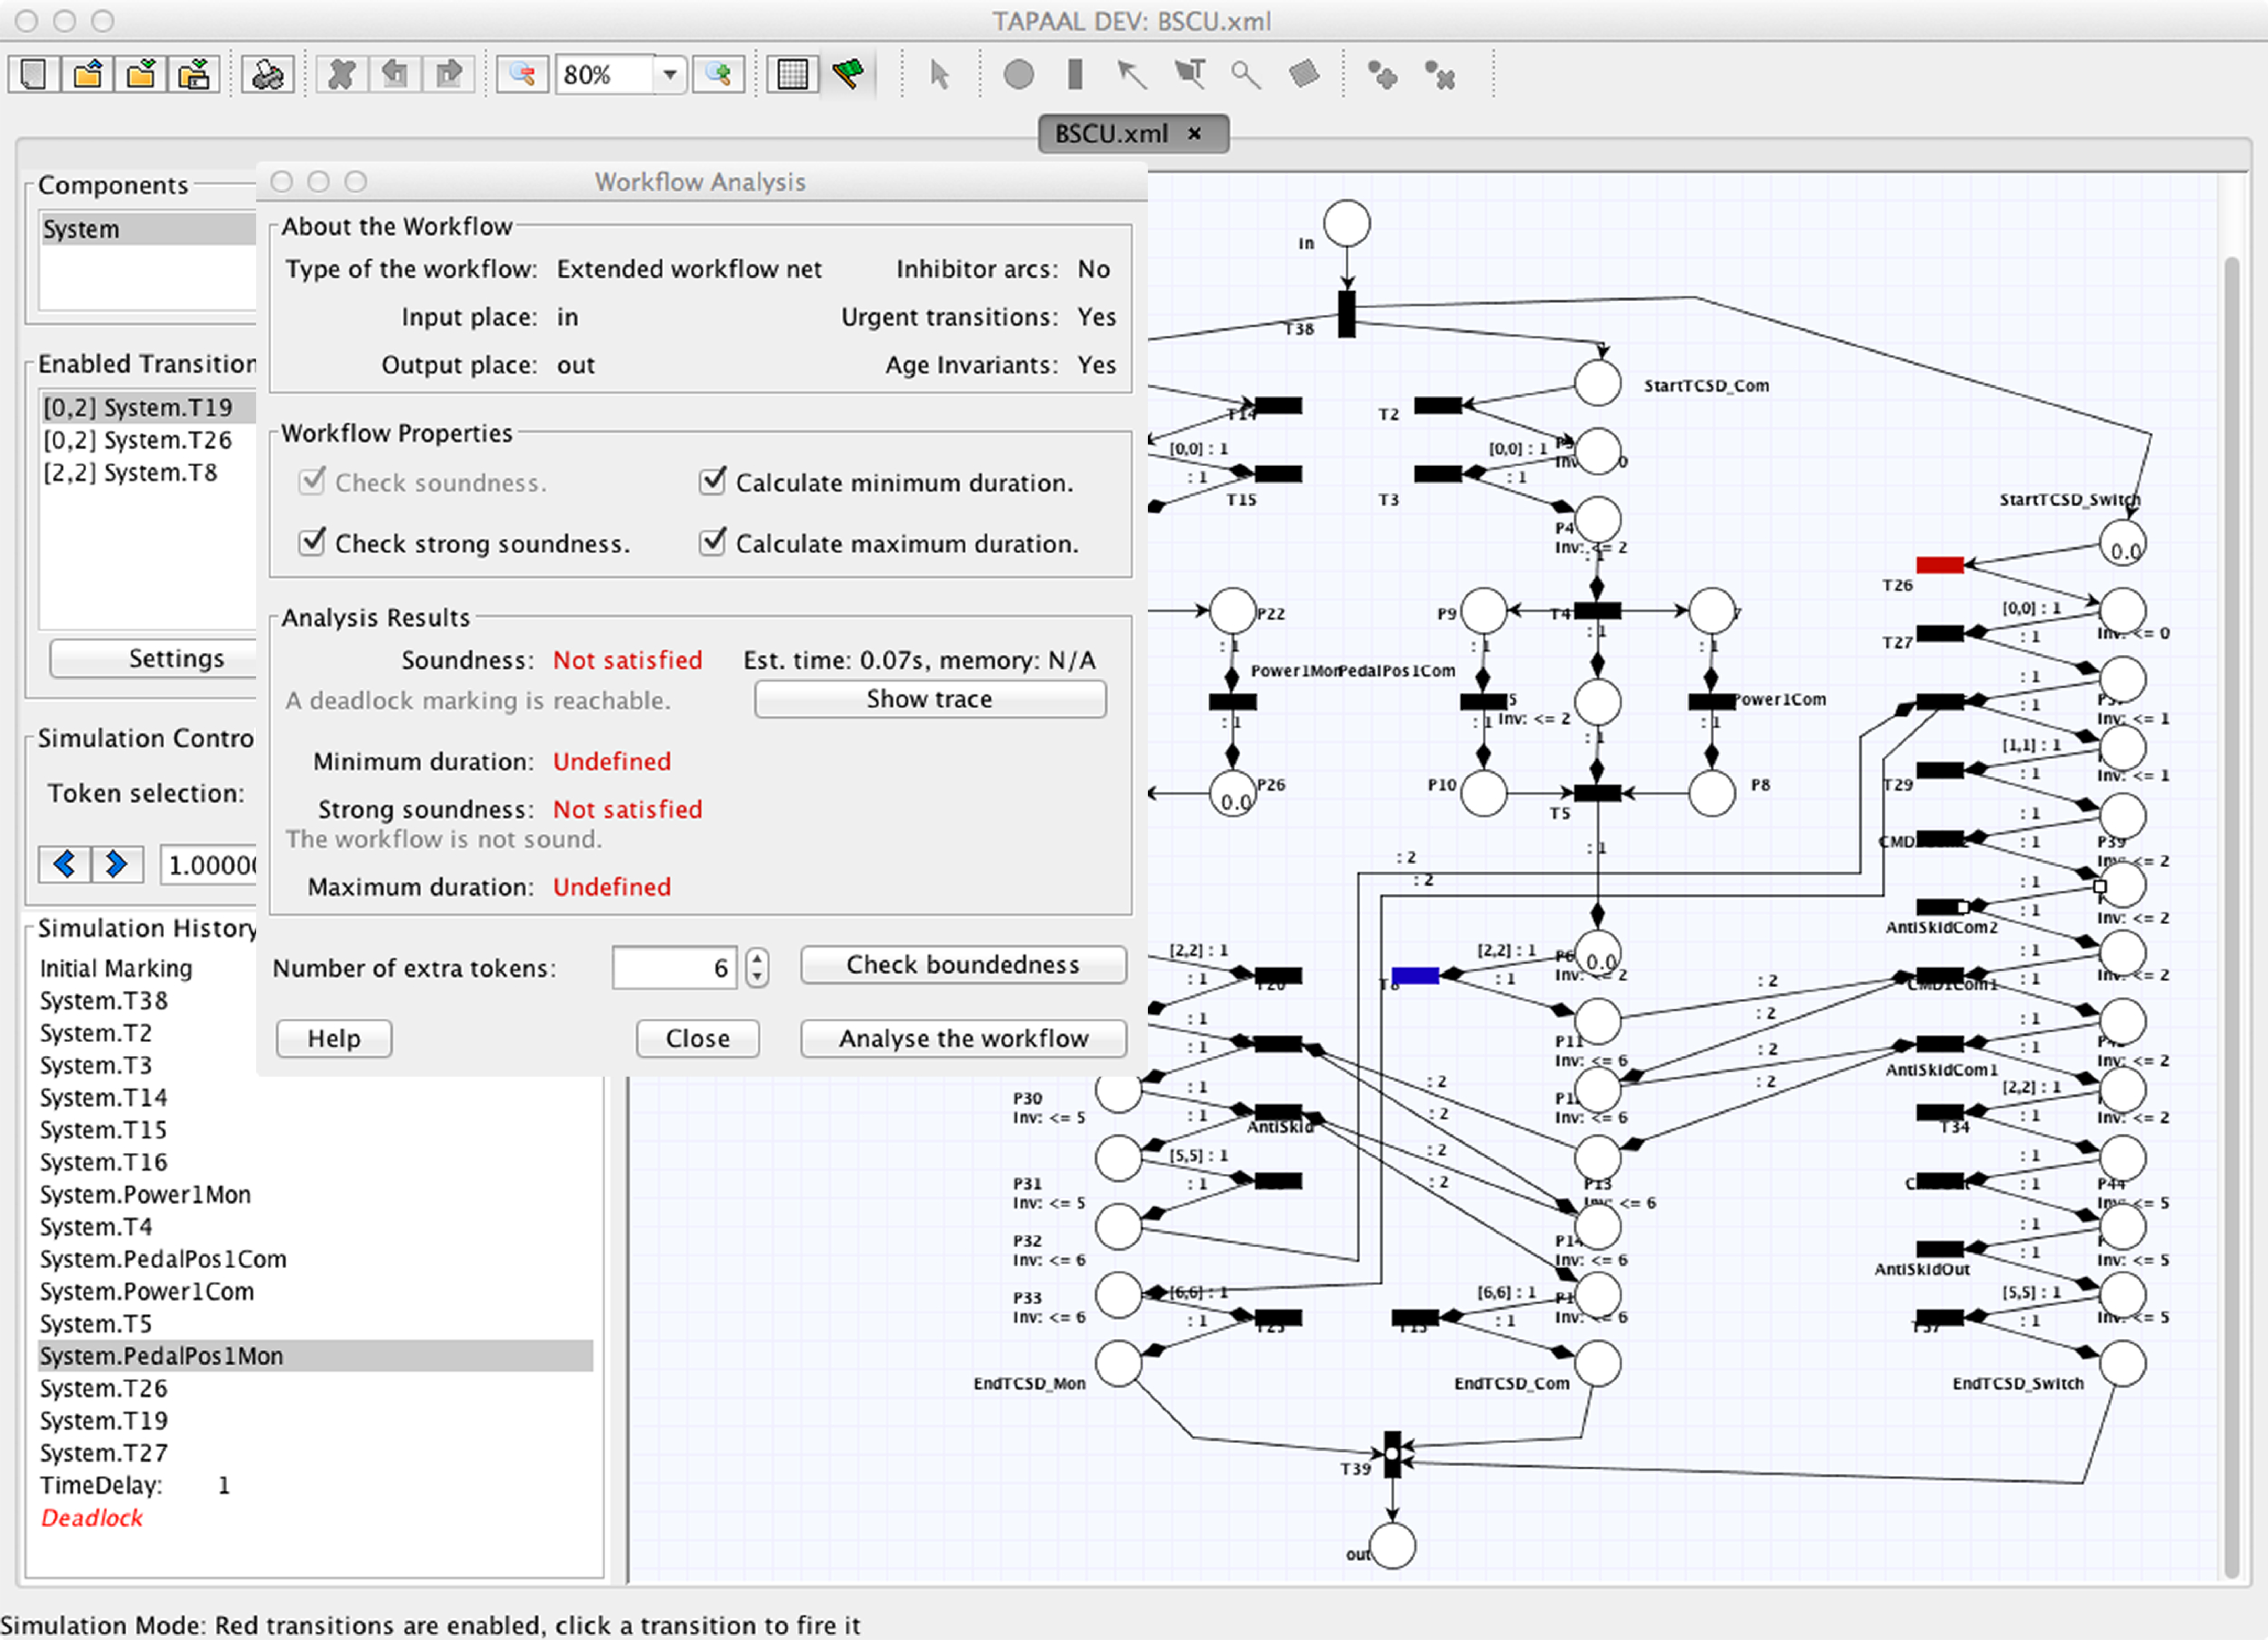
\includegraphics[width=1\textwidth]{Figures/screenshot-combined.eps}
\end{center}
\caption{Screenshot of the workflow analysis tool}
\label{fig:screenshot}
\end{figure}

In the Brake System Control Unit (BSCU) case study, a part of a 
Wheel Braking System (WBS) used for the certification of civil aircrafts 
in the SAE standard ARP4761~\cite{SEB:FESCA:13}, we discovered  
in less than 1 second that the workflow is not sound due to 
unexpected deadlocks. The authors of~\cite{SEB:FESCA:13} 
were able to detect these problems asking a reachability query,
however, the error traces contradicting soundness were constructed
manually. Our implementation allows a fully automatic detection and
visualization of such situations.

In the second case study describing the workflow of MPEG2 encoding algorithm
run on a multicore processor (Petri net model was taken 
from~\cite{PCVMP:MMM:04}), we verified in about 10 seconds 
both soundness and strong soundness, and computed 
the minimum and maximum encoding time for the IBBP frame sequence.

In the third case study, we checked the soundness 
of a larger blood transfusion workflow~\cite{blood-benchmark},
the benchmarking case study of the little-JIL language. 
The Petri net model was suggested in~\cite{BLS:FHIES:12} but we discovered 
several issues with improper workflow termination that were fixed
and then both soundness and strong soundness was confirmed
in about 1 second, including the information about the minimum 
and maximum execution times. 

TAPAAL models of all case studies can be obtained from www.tapaal.net
and Figure~\ref{fig:screenshot} shows a screenshot of the GUI in the
trace debugging mode for workflow analysis of the brake system control 
unit mentioned above.

\section{Summary}\label{sumWorkflow}
\markright{~\ref{sumWorkflow} Summary}

We have presented in this chapter a framework for modelling timed workflow processes
via timed-arc workflow nets and studied the classical problem of
soundness and its extension to time-bounded (strong) soundness.
We provided a comprehensive analysis of decidability/undecidability
of soundness and strong soundness on different subclasses of timed-arc
workflow nets. We also suggested efficient algorithms for computing
minimum and maximum execution times of a given workflow and implemented
all algorithms within the tool TAPAAL. 
As a result we have a complete theory for checking soundness on
timed workflow nets and contrary to many other works studying
different variants of workflow processes, we took a step further
by providing efficient implementation of the algorithms, including
a platform independent GUI support for modular design of timed
workflow nets and visual error trace debugging. The tool is open-source
and freely available at \url{www.tapaal.net}.
The practical usability of 
the approach was documented on three industry-inspired case studies,
demonstrating a very promising potential for verification of larger
timed workflows.

In the study we focused on the discrete semantics 
of workflow nets that is often sufficient and allows for modelling
of workflows where events can happen in discrete steps.
Nevertheless, we argued that many of the results
are valid also for the continuous semantics. In fact, once we
know that a given net is sound in the continuous semantics,
it is enough to check for strong soundness and minimum/maximum
execution times in the discrete semantics and these answers
are valid also for the continuous case. As a future work, we 
are developing efficient algorithms to decide soundness 
of bounded timed-arc workflow nets in the continuous semantics.